% -*- mode: latex; mode: reftex; mode: auto-fill; mode: flyspell; mode: yas/minor; coding: utf-8; tex-command: "pdflatex.sh" -*-

%% \PassOptionsToClass{handout}{beamer}

\documentclass[c,8pt]{beamer}

\usepackage[utf8]{inputenc}
\usepackage{overpic}
\usepackage{pgfplots}
\usepackage{xspace}
\usepackage{verbatimbox} % To insert verbatim inside \note

%%%%%%%%%%%%%%%%%%%%%%%%%%%%%%%%%%%%%%%%%%%%%%%%%%%%%%%%%%%%%%%%%%%%%%

%% \bibliographystyle{abbrvnat}
\bibliographystyle{includes/abbrvnatforbeamer}
\usepackage{multirow}

\usepackage{microtype}
\usepackage{amsmath}
\usepackage{amssymb}
\usepackage{dsfont}
\usepackage{verbatim}
\usepackage{upquote}
\usepackage{anyfontsize}
\usepackage[round]{natbib}
\usepackage{fancyvrb}
\usepackage{mathtools}
\usepackage{etex}
\usepackage{xparse}
\usepackage{xifthen}
%% \usepackage{BOONDOX-cal}

\def\theurl{\url{https://fleuret.org/dlc/}}
\def\theauthor{Fran\c cois Fleuret}
\def\coursetitle{Deep learning}

\makeatletter
\DeclareFontEncoding{LS1}{}{}
\DeclareFontSubstitution{LS1}{stix}{m}{n}
\DeclareMathAlphabet{\mathcal}{LS1}{stixscr}{m}{n}
\makeatother

\def\relu{\operatorname{ReLU}}
\def\softmax{\operatorname{softmax}}
\def\sigmoid{\operatorname{sigm}}
\def\sample{\operatorname{sample}}
\def\diag{\operatorname{diag}}
\def\sign{\operatorname{sign}}
\def\argmax{\operatornamewithlimits{argmax}}
\def\argmin{\operatornamewithlimits{argmin}}
\def\trace{\operatorname{Tr}}

% Olivier: I changed {\it #1} to \textit{#1} because there are
% different and does not mess up with serif/sansserif
%
% https://tex.stackexchange.com/questions/8053/is-there-a-difference-between-textit-and-itshape
\newcommand{\latin}[1]{\textit{#1}}
% \newcommand{\latin}[1]{{\it #1}}

\newcommand{\materialsurl}[1]{\url{https://fleuret.org/dlc/#1}}

\newcommand{\DATAVAR}{\mathbf{{\cal D}}}
\newcommand{\DATAVAL}{\mathbf{d}}
\newcommand{\BD}{\mathbf{D}}
\newcommand{\LL}{\mathcal{L}}
\newcommand{\Ll}{\mathcal{l}}
\newcommand{\RR}{\mathbb{R}}
\newcommand{\Lh}{\mathcal{h}}
\newcommand{\transpose}{^{\top}}

\newcommand{\dd}[2]{\frac{\partial {#1}}{\partial {#2}}}
%%\newcommand{\jacob}[2]{\left[ \dd{#1}{{#2}} \right]}
\newcommand{\gradient}[2]{\left[ \dd{#1}{{#2}} \right]}
%% \newcommand{\jacob}[2]{\mathbf{J}_{#1}}
\newcommand{\DD}[2]{\left[ \frac{\partial {#1}}{\partial {#2}} \right]}
\newcommand{\lbb}{\left[\!\!\left[}
\newcommand{\rbb}{\right]\!\!\right]}

\newcommand{\parname}[1]{{(#1)}}
\newcommand{\naming}[1]{{\text{(#1)}}}

%% \newcommand{\parname}[1]{{\vec{#1}}}
%% \newcommand{\parname}[1]{{\widetilde{#1}}}
%% \newcommand{\parname}[1]{{\tilde{#1}}}
%% \newcommand{\parname}[1]{{(#1)}}

%% \DeclareMathOperator*{\expect}{\mathds{E}}
%% \DeclareMathOperator*{\variance}{\mathds{V}}
%% \DeclareMathOperator*{\empexpect}{\hat{\mathds{E}}}
%% \DeclareMathOperator*{\mutinf}{\mathds{I}}
%% \DeclareMathOperator*{\empmutinf}{\hat{\mathds{I}}}
%% \DeclareMathOperator*{\entropy}{\mathds{H}}
%% \DeclareMathOperator*{\empentropy}{\hat{\mathds{H}}}

\def\given{\,\middle\vert\,}
\newcommand{\proba}{{P}}
\newcommand{\seq}{{S}}
%% \newcommand{\proba}{\mathds{P}}
\newcommand{\expect}{\mathds{E}}
\newcommand{\variance}{\mathds{V}}
\newcommand{\empexpect}{\hat{\mathds{E}}}
\newcommand{\mutinf}{\mathds{I}}
\newcommand{\empmutinf}{\hat{\mathds{I}}}
\newcommand{\entropy}{\mathds{H}}
\newcommand{\empentropy}{\hat{\mathds{H}}}
\newcommand{\ganG}{\mathbf{G}}
\newcommand{\ganD}{\mathbf{D}}
\newcommand{\ganF}{\mathbf{F}}

\newcommand{\dkl}{\mathds{D}_{\mathsf{KL}}}
\newcommand{\djs}{\mathds{D}_{\mathsf{JS}}}

\newcommand*{\vertbar}{\rule[-1ex]{0.5pt}{2.5ex}}
\newcommand*{\horzbar}{\rule[.5ex]{2.5ex}{0.5pt}}

\usepackage{xcolor}

%%%%%%%%%%%%%%%%%%%%%%%%%%%%%%%%%%%%%%%%%%%%%%%%%%%%%%%%%%%%%%%%%%%%%%
%% Colors

\definecolor{blue}{rgb}{0.0,0.0,0.55}
\definecolor{paleblue}{rgb}{0.50,0.50,1.00}
\definecolor{darkblue}{rgb}{0.10,0.10,0.70}

\definecolor{red}{rgb}{1.0,0.0,0.0}
\definecolor{palered}{rgb}{1.00,0.50,0.50}
\definecolor{darkred}{rgb}{0.75,0.0,0.0}

\definecolor{green}{rgb}{0.0,0.50,0.0}
\definecolor{palegreen}{rgb}{0.5,1.00,0.5}
\definecolor{darkgreen}{rgb}{0.0,0.5,0.0}

\definecolor{dimmed}{rgb}{0.8,0.8,0.8}

\definecolor{orange}{rgb}{1.0,0.6,0.0}
\definecolor{bluegray}{rgb}{0.1,0.2,0.7}

\newcommand{\blue}{\color{blue}}
\newcommand{\darkblue}{\color{darkblue}}
\newcommand{\paleblue}{\color{paleblue}}
\newcommand{\green}{\color{green}}
\newcommand{\darkgreen}{\color{darkgreen}}
\newcommand{\palegreen}{\color{palegreen}}
\newcommand{\red}{\color{red}}
\newcommand{\darkred}{\color{darkred}}
\newcommand{\palered}{\color{palered}}
\newcommand{\black}{\color{black}}

%%%%%%%%%%%%%%%%%%%%%%%%%%%%%%%%%%%%%%%%%%%%%%%%%%%%%%%%%%%%%%%%%%%%%%

\newcommand{\quotepaper}[2]{%
\begin{center}%
%
\begin{minipage}{0.95\textwidth}
``#2''
\end{minipage}%
%
\end{center}

\vspace*{-1ex}

\acksource{\citep{#1}}
}

%%%%%%%%%%%%%%%%%%%%%%%%%%%%%%%%%%%%%%%%%%%%%%%%%%%%%%%%%%%%%%%%%%%%%%

\newcommand{\quotesource}[2]{%
\begin{center}%
%
\begin{minipage}{0.95\textwidth}
``#2''
\end{minipage}%
%
\end{center}

\vspace*{-1ex}

\acksource{#1}
}

%%%%%%%%%%%%%%%%%%%%%%%%%%%%%%%%%%%%%%%%%%%%%%%%%%%%%%%%%%%%%%%%%%%%%%

\definecolor{codecolor}{rgb}{0.0,0.0,0.0}
\definecolor{codecolor2}{rgb}{0.0,0.0,0.0}

%% One keyword. The heavy magic to allow the percent symbol
%% \makeatletter
%% \newcommand{\kw}{\catcode`\%=12\@kw}
%% \DeclareRobustCommand{\@kw}[1]{{{\color{codecolor}\tt \detokenize{#1}}\catcode`\%=14}{}}
%% \makeatother
\DeclareRobustCommand{\kw}[1]{{\color{codecolor}\tt \detokenize{#1}}}

%% Inline piece of code

\DefineVerbatimEnvironment{rawsrc}{BVerbatim}{fontsize=\small,baselinestretch=1.0,formatcom=\color{codecolor}}

%% Sub-part of a file

\ifnum\pdfshellescape=1
\NewDocumentCommand{\rawsrcexcerpt}{mmmO{}O{1}}{%
  \BVerbatimInput[fontsize=\small,baselinestretch=1.0,formatcom=\color{codecolor},#4]{|"< #1 awk '/#2/{flag=1;next}/#3/{flag=0}flag {print substr($0, #5)}' | grep -v HIDE_IN_SLIDE"}%
}
\else
\NewDocumentCommand{\rawsrcexcerpt}{mmmO{}O{1}}{%
  {\color{darkred} \tt Source snippet omitted because shell escape is disabled.}%
}
\fi

%%%%%%%%%%%%%%%%%%%%%%%%%%%%%%%%%%%%%%%%%%%%%%%%%%%%%%%%%%%%%%%%%%%%%%

\newenvironment{warning}{%
\raisebox{-8pt}{%
\begin{tikzpicture}[scale=0.6]
\node at (0, 0) {\huge\textrm{\textbf{!}}};
\draw[rounded corners=1pt,line width=1.5pt,darkred] (-0.6, -0.47) -- ++(1.2, 0) -- ++(-0.6, 1.2) -- cycle;
\end{tikzpicture}%
}%
%% {\darkred \huge {\fontencoding{U}\fontfamily{futs}\selectfont\char 66\relax}}%
%
\hspace*{0.75em}%
%
\begin{minipage}{0.9\textwidth}
}{%
\end{minipage}%
}

%%%%%%%%%%%%%%%%%%%%%%%%%%%%%%%%%%%%%%%%%%%%%%%%%%%%%%%%%%%%%%%%%%%%%%

\newcommand{\fixedheightbox}[2]{%
   \sbox{0}{\parbox{\textwidth}{#2}}
    \ifdim\dimexpr\ht0+\dp0<#1
    \dp0\dimexpr#1-\ht0\fi
    \usebox{0}%
}

\makeatletter
\newcommand{\smallerthantiny}{\@setfontsize{\smallerthantiny}{4pt}{5pt}}
\makeatother

%%%%%%%%%%%%%%%%%%%%%%%%%%%%%%%%%%%%%%%%%%%%%%%%%%%%%%%%%%%%%%%%%%%%%%
%% The \draft command

\newcounter{nbdrafts}
\setcounter{nbdrafts}{0}
\makeatletter
\newcommand{\checknbdrafts}{
\ifnum \thenbdrafts > 0
\@latex@warning@no@line{**********************************************************************}
\@latex@warning@no@line{* The document contains \thenbdrafts \space draft note(s)}
\@latex@warning@no@line{**********************************************************************}
\fi}
\newcommand{\draft}[1]{\addtocounter{nbdrafts}{1}{\color{red} #1}}
\makeatother

\newcommand{\vstretch}{\vspace*{\stretch{1}}}
\newcommand{\hstretch}{\hspace*{\stretch{1}}}

%%%%%%%%%%%%%%%%%%%%%%%%%%%%%%%%%%%%%%%%%%%%%%%%%%%%%%%%%%%%%%%%%%%%%%
% Across files references, e.g. \dlclabel{autograd} in the slide file
% about autograd, and \dlcref{autograd} where we want to refer to it

\newcommand{\dlclabel}[1]{%
\newwrite\file
\immediate\openout\file=#1.dlcref
%% \immediate\write\file{\dlclecturenumber.\dlcdecknumber.\,``\detokenize\expandafter{\dlcdecktitle}''}
%\immediate\write\file{\dlclecturenumber.\dlcdecknumber.\detokenize\expandafter{\,``\dlcdecktitle''}}
\immediate\write\file{\dlclecturenumber.\dlcdecknumber. ``\dlcdecktitle''}
\immediate\closeout\file
}

\newcommand{\dlcref}[1]{%
\InputIfFileExists{#1.dlcref}{}{[dlcref #1 undefined]}\unskip
%\@input{#1.dlcref}\unskip
}%

%%%%%%%%%%%%%%%%%%%%%%%%%%%%%%%%%%%%%%%%%%%%%%%%%%%%%%%%%%%%%%%%%%%%%%

% To include a .pdf image which itself includes a raster image
% relative to itself
%
% https://tex.stackexchange.com/a/282110
\newcommand\inputpgf[2]{{
\let\pgfimageWithoutPath\pgfimage
\renewcommand{\pgfimage}[2][]{\pgfimageWithoutPath[##1]{#1/##2}}
\input{#1/#2}
}}


\usepackage{tikz}

\usetikzlibrary{positioning,fit,backgrounds}
\usetikzlibrary{arrows.meta,decorations.pathreplacing}
\usetikzlibrary{calc}
\usetikzlibrary{shapes,calc,intersections}
\usetikzlibrary{patterns}
%% \usetikzlibrary{shapes.multipart}

\usetikzlibrary{arrows}
%% \tikzset{>=angle 90}

\definecolor{nn-data}   {rgb}{0.90, 0.95, 1.00}
\definecolor{nn-param}  {rgb}{1.00, 0.90, 0.50}
\definecolor{nn-process}{rgb}{0.80, 1.00, 0.80}

\tikzset{
  pics/box/.style args={#1/#2/#3/#4/#5/#6}{
    code={
      \pgfmathsetmacro{\slant}{0.35}
      \pgfmathsetmacro{\width}{#1}
      \pgfmathsetmacro{\height}{#2}
      \pgfmathsetmacro{\thickness}{#3}
      \pgfmathsetmacro{\lwidth}{#4}
      \pgfmathsetmacro{\lheight}{#5}
      \pgfmathsetmacro{\lthickness}{#6}
      \pgfmathsetmacro{\labelgap}{0.15}

      \pgfmathsetmacro{\centerx}{0}
      \pgfmathsetmacro{\centery}{\height * 0.5 + \width * 0.5 * \slant}

      % Filled body

      \draw[fill] ( - \centerx, - \centery)
      -- ++(0.0, \height)
      -- ++(\slant * 0.5 * \width, 0.5 * \width)
      -- ++(\thickness, 0.0)
      -- ++(0, -\height)
      -- ++(- \slant * 0.5 * \width, -0.5 * \width)
      -- ++(-\thickness, 0)
      ;

      % Additional edges

      \draw  ( - \centerx, - \centery) ++(0.0, \height)
      -- ++(\thickness, 0.0) -- ++(\slant * 0.5 * \width, 0.5 * \width)
      ;

      \draw  ( - \centerx, - \centery) ++(\thickness, \height)
      -- ++(0.0, -\height)
      ;

      % Axis length labels

      \ifthenelse
      {\equal{\lwidth}{}}{}
      {
        \draw[<->]  ( - \centerx, - \centery) ++(0.0, \height) ++(-\labelgap * .7071, \labelgap * .7071)
        -- ++(\slant * 0.5 * \width, 0.5 * \width) node[midway, above left] {\scriptsize \lwidth};
      }

      \ifthenelse
      {\equal{\lheight}{}}{}
      {
        \draw[<->]  ( - \centerx, - \centery) ++(-\labelgap, 0.0)
        -- ++(0.0, \height) node[midway, left] {\scriptsize \lheight};
      }

      \ifthenelse
      {\equal{\lthickness}{}}{}
      {
        \draw[<->]  ( - \centerx, - \centery) ++(0.0, -\labelgap)
        -- ++(\thickness, 0.0) node[midway, below] {\scriptsize \lthickness};
      }

      % Anchor points

      \coordinate (-center) at (\thickness + \slant * 0.25 * \width, 0.0);

      \coordinate (-follow-tight) at (\thickness + 0.2, 0.0);

      \coordinate (-follow-close) at (\thickness + \slant * 0.5 * \width, 0.0);

      \coordinate (-follow) at (\thickness + \slant * 0.2 * \width + 1.0, 0.0);

      \coordinate (-above-back)  at (-\centerx + \slant * 0.5 * \width + \thickness * 0.5, \height - \centery + 0.5 * \width + 0.3);

      \coordinate (-above)  at (-\centerx + \thickness * 0.5, \height - \centery + 0.5 * \width + 0.3);

      \coordinate (-below)  at (-\centerx + \thickness * 0.5, -\centery - 0.5);
    }
  },
  pics/box/.default=0.5/1/1/1/1/1
}

%%%%%%%%%%%%%%%%%%%%%%%%%%%%%%%%%%%%%%%%%%%%%%%%%%%%%%%%%%%%%%%%%%%%%%

%% \newcommand{\intint}[1]{[\![#1]\!]}
\newcommand{\intint}[1]{[\![#1]\!]}

\newcommand{\cube}[6]{
    \draw[#1,#2] #3 -- ++#4 -- ++#5 -- ++#6 -- ++($(0, 0) - #4$) -- ++($(0, 0) - #5$) -- ++($(0, 0) - #6$);
    \draw[#1] #3 ++#4 -- ++#6 -- ++#5;
    \draw[#1] #3 ++#6 -- ++#4;
}

%%%%%%%%%%%%%%%%%%%%%%%%%%%%%%%%%%%%%%%%%%%%%%%%%%%%%%%%%%%%%%%%%%%%%%

\newcommand{\oneconv}[3]{
  \uncover<#1>{
    \cube{draw=black,thick}{fill=black!15}{#3}{(0, 1)}{(0.4, 0.8)}{(1, 0)}
  }

  \uncover<#1-#2>{
    \cube{draw=green,thick}{fill=white}{#3 ++(7.4, 0.4)}{(0, 0.6)}{(0.2, 0.4)}{(0.33333, 0)}
  }
}

\newcommand{\onepool}[3]{
  \uncover<#1>{
    \cube{draw=black,thick}{fill=black!15}{#3}{(0, 1)}{(0.4, 0.8)}{(1, 0)}
  }

  \uncover<#1-#2>{
    \cube{draw=green,thick}{fill=white}{#3 ++(7.4, 0.4)}{(0, 0.6)}{(0.2, 0.4)}{(0.33333, 0)}
  }
}

%%%%%%%%%%%%%%%%%%%%%%%%%%%%%%%%%%%%%%%%%%%%%%%%%%%%%%%%%%%%%%%%%%%%%%

\newcommand{\drawvector}[1]{
%% \raisebox{0.75cm}{\Large $\Bigg($}
\begin{tikzpicture}[scale=0.2]
  \draw[draw=none] (0, -4) -- (0, 4);
  \edef\xdraw{0}
  \draw[black!20,thin] (0, -0.2) -- ++(0, 0.4);
  \foreach \y in { #1 }{
    \pgfmathparse{\xdraw+1}
    \xdef\xdraw{\pgfmathresult}
    \draw[black!20,thin] (\xdraw, -0.2) -- ++(0, 0.4);
  }
  \draw[black!20,thin] (-0.1, 0) -- (\xdraw, 0) ++(0.1, 0);
  \edef\xdraw{0}
  \foreach \y in { #1 }{
    \draw[] (\xdraw, 0) -- ++(0, \y) -- ++(1.0, 0.0) -- ++(0, -\y);
    %% \draw[] (\xdraw, \y) -- ++(0.05, 0) -- ++(0.9, 0.0);
    %% \draw[thick] (\xdraw,\y) +(0.05, 0) -- ++(0.9, 0.0);
    \pgfmathparse{\xdraw+1}
    \xdef\xdraw{\pgfmathresult}
  }
\end{tikzpicture}%
%% \raisebox{0.75cm}{\Large $\Bigg)$}
}

%%%%%%%%%%%%%%%%%%%%%%%%%%%%%%%%%%%%%%%%%%%%%%%%%%%%%%%%%%%%%%%%%%%%%%

%%%%%%%%%%%%%%%%%%%%%%%%%%%%%%%%%%%%%%%%%%%%%%%%%%%%%%%%%%%%%%%%%%%%%%
% A command to illustrate the convolutional layer output size

\newcommand{\convscheme}[4]{
\begin{tikzpicture}[scale=0.15]
\draw (0, 0) -- (#1, 0);
\draw[<->] (0, 1.75) -- ++(#1, 0) node[midway,above] {$#1$};

\draw[fill=green!25] (#1, 0.00) ++(-#2, 0.0) rectangle ++(#2, 1.0);

\foreach \x in { 1,...,#1 }
  \draw[thin] (\x, 0.0) ++(-1, 0) rectangle ++(1, 1);

\draw[] (0, 0.00) ++(0, -0.5) -- ++({#3*(#4-1)+1}, 0.0) node[midway,below] {$\times #4$};

\foreach \x in { 1,...,#4 }
  \draw[fill=black] ({#3*(\x-1)}, 0.5) ++(0.5, 0) circle(4pt);
\end{tikzpicture}
}

\newcommand{\convtransposescheme}[4]{
\begin{tikzpicture}[scale=0.15]
\draw (0, 0) -- (#1, 0);

\draw[fill=green!25] (#1, 0.00) ++(-#2, 0.0) rectangle ++(#2, 1.0);

\foreach \x in { 1,...,#1 }
  \draw[thin] (\x, 0.0) ++(-1, 0) rectangle ++(1, 1);

\draw[] (0, 0.00) ++(0, 1.5) -- ++({#3*(#4-1)+1}, 0.0) node[midway,above] {$\times #4$};
%% \draw[<->] (#1, 0.00) ++(-#2, -0.75) -- ++(#2, 0.0) node[midway,below] {$#2$};
\draw[<->] (0, -0.75) -- ++(#1, 0.00) node[midway,below] {$#1$};

\foreach \x in { 1,...,#4 }
  \draw[fill=black] ({#3*(\x-1)}, 0.5) ++(0.5, 0) circle(4pt);
\end{tikzpicture}
}

%%%%%%%%%%%%%%%%%%%%%%%%%%%%%%%%%%%%%%%%%%%%%%%%%%%%%%%%%%%%%%%%%%%%%%

\tikzset{>={Straight Barb[angle'=80,scale=1.1]}}

\tikzset{
  value/.style    ={ font=\scriptsize, rectangle, draw=black!50, fill=white,   thick,
                     inner sep=3pt, inner xsep=2pt, minimum size=10pt, minimum height=20pt },
  parameter/.style={ font=\scriptsize, rectangle, draw=black!50, fill=blue!15, thick,
                     inner sep=0pt, inner xsep=2pt, minimum size=10pt, minimum height=20pt },
  operation/.style={ font=\scriptsize, rectangle,    draw=black!50, fill=green!30, thick,
                     inner sep=3pt, minimum size=10pt, minimum height=20pt },
  flow/.style={->,shorten <= 1pt,shorten >= 1pt, draw=black!50, thick},
%
  f2f/.style={draw=black!50, thick},
  v2f/.style={{Bar[width=1.5mm]}-,shorten <= 0.75pt,draw=black!50, thick},
  f2v/.style={->,shorten >= 0.75pt,draw=black!50, thick},
  v2v/.style={{Bar[width=1.5mm]}->,shorten <= 0.75pt,shorten >= 0.5pt,draw=black!50, thick},
%
%
  df2f/.style={draw=black, thick},
  dv2f/.style={{Bar[width=1.5mm]}-,shorten <= 0.75pt,draw=black, thick},
  df2v/.style={->,shorten >= 0.75pt,draw=black, thick},
  dv2v/.style={{Bar[width=1.5mm]}->,shorten <= 0.75pt,shorten >= 0.5pt,draw=black, thick},
%
  differential/.style    ={ font=\small, rectangle, draw=black!50,               thick,
                     inner sep=3pt, inner xsep=2pt, minimum size=10pt, minimum height=20pt, fill=yellow!80 },
  dflow/.style={->,shorten <= 1pt,shorten >= 1pt, draw=black, thick}
}

\newcommand{\nophone}{
\begin{tikzpicture}

\draw[fill=black] (0, 0) to (0, 7) to [out=6,in=174] (4, 7) to (4, 0) to [out=186,in=354] (0, 0);

\draw[fill=white] (0.2, 0.75) rectangle (3.8, 6.35);
\draw[fill=white] (2, 0.27) circle (0.2);
\draw[fill=white] (1, 6.7) circle (0.1);

\draw[line width=33pt,color=white] (2, 3.5) circle (5cm);
\draw[line width=33pt,color=white] (2, 3.5) ++(-3.3, -3.3) -- ++(6.6, 6.6);
\draw[line width=23pt,color=red] (2, 3.5) circle (5cm);
\draw[line width=23pt,color=red] (2, 3.5) ++(-3.3, -3.3) -- ++(6.6, 6.6);

\end{tikzpicture}
}

%\input{includes/source-highlight}

\pgfplotsset{compat=1.11}

%%%%%%%%%%%%%%%%%%%%%%%%%%%%%%%%%%%%%%%%%%%%%%%%%%%%%%%%%%%%%%%%%%%%%%
%% The witharrows mess due to my old Debian

\usepackage{witharrows} % To make explanatory arrows between equation lines

%% \usepackage{environ}
%% \NewEnviron{DispWithArrows*}{%
%% \begin{align}
%% \BODY
%% \end{align}
%% }
%% \newcommand{\Arrow}[1]{}

%%%%%%%%%%%%%%%%%%%%%%%%%%%%%%%%%%%%%%%%%%%%%%%%%%%%%%%%%%%%%%%%%%%%%%
%% Do not skip frame numbers
\usepackage{etoolbox}
\makeatletter
\pretocmd{\beamer@@@@frame}{\alt<#1>{}{\beamer@noframenumberingtrue}}{}{}
\makeatother
%%%%%%%%%%%%%%%%%%%%%%%%%%%%%%%%%%%%%%%%%%%%%%%%%%%%%%%%%%%%%%%%%%%%%%

%%%%%%%%%%%%%%%%%%%%%%%%%%%%%%%%%%%%%%%%%%%%%%%%%%%%%%%%%%%%%%%%%%%%%%
% To make an index
\newenvironment{theindex}{}{}
\usepackage{imakeidx}
\usepackage{fp}

\makeatletter
% Global redefinition of indexentry to use section, then page
\newcounter{tmpcounter}
\renewcommand{\imki@wrindexentrysplit}[3]{%
  %%%%%%%%%%%%%%%%%%%%%%%%%%%%%%%%%%%%%%%%%%%%%%%%%%%
  % To make the items easily sortable (integers) without redefining too
  % much xindy and co. an index is referenced with:
  % 13002007 : lecture 13, course 2, frame 7
  % 1000000 * lecture + 1000 * deck + frame
  %%%%%%%%%%%%%%%%%%%%%%%%%%%%%%%%%%%%%%%%%%%%%%%%%%%
  % End all following lines with '%' otherwise,
  % an extra space is generated by \index
  %%%%%%%%%%%%%%%%%%%%%%%%%%%%%%%%%%%%%%%%%%%%%%%%%%%
  \setcounter{tmpcounter}{\dlclecturenumber}%
  \ifnum \thetmpcounter > 999%
  \PackageError{dlc}{Lecture number (\dlclecturenumber) should be < 1000 for index encoding}{}%
  \fi%
  \setcounter{tmpcounter}{\dlcdecknumber}%
  \ifnum \thetmpcounter > 999%
  \PackageError{dlc}{Deck number (\dlcdecknumber) should be < 1000 for index encoding}{}%
  \fi%
  \FPeval{\indexid}{clip(1000000*\dlclecturenumber+1000*\dlcdecknumber+\insertframenumber)}%
  % \expandafter\protected@write\csname#1@idxfile\endcsname{}{\string\indexentry{#2}{\lecturenumber.\coursenumber:\insertframenumber}}%
  \expandafter\protected@write\csname#1@idxfile\endcsname{}{\string\indexentry{#2}{\indexid}}%
}%
\makeatother
%%%%%%%%%%%%%%%%%%%%%%%%%%%%%%%%%%%%%%%%%%%%%%%%%%%%%%%%%%%%%%%%%%%%%%

\makeindex

\let\oldindex\index % save old definition to prevent recursion
\renewcommand*\index[1]{\oldindex{#1|formatsliderange}}
% \renewcommand*\index[1]{\oldindex{#1|formatsliderange}\ignorespaces}
%%%%%%%%%%%%%%%%%%%%%%%%%%%%%%%%%%%%%%%%%%%%%%%%%%%%%%%%%%%%%%%%%%%%%%


% %%~~~~~~~~~~~~~~~~~~~~~~~~~~~~~~~~~~~~~~~~~~~~~~~~~~~~
% \mode<handout>{
%   \usepackage{pgfpages}
%   %% \pgfpagesuselayout{16 on 1}[a4paper,border shrink=0mm,landscape]
%   %% \pgfpageslogicalpageoptions{1}{border code=\pgfusepath{stroke}}
%   %% \pgfpageslogicalpageoptions{2}{border code=\pgfusepath{stroke}}
%   %% \pgfpageslogicalpageoptions{3}{border code=\pgfusepath{stroke}}
%   %% \pgfpageslogicalpageoptions{4}{border code=\pgfusepath{stroke}}
%   \pgfpagesuselayout{2 on 1}[a4paper,border shrink=4mm]
% }
% %% \setbeamercovered{transparent}
% %%~~~~~~~~~~~~~~~~~~~~~~~~~~~~~~~~~~~~~~~~~~~~~~~~~~~~

%%~~~~~~~~~~~~~~~~~~~~~~~~~~~~~~~~~~~~~~~~~~~~~~~~~~~
\usepackage{makecell}
%% To get handout on top of A4 page and not below, and to handle the
%% fact that some slides don't have notes.

\usepackage{ragged2e}  % justify text

\mode<handout>{
  % \setbeamercolor{background canvas}{bg=gray!10} % Olivier: debug handout
  \usepackage{pgfpages}
  %% \pgfpagesuselayout{16 on 1}[a4paper,border shrink=0mm,landscape]
  %% \pgfpageslogicalpageoptions{1}{border code=\pgfusepath{stroke}}
  %% \pgfpageslogicalpageoptions{2}{border code=\pgfusepath{stroke}}
  %% \pgfpageslogicalpageoptions{3}{border code=\pgfusepath{stroke}}
  %% \pgfpageslogicalpageoptions{4}{border code=\pgfusepath{stroke}}
  \pgfpagesuselayout{2 on 1}[a4paper,border shrink=3mm]

  \ifdefined\withoutnotes
    \ifdefined\withnotes
      \setbeameroption{show notes}
    \fi
  \else
    \setbeameroption{show notes}
    %% \pgfpageslogicalpageoptions{1}{border code=\pgfusepath{stroke}}
  \fi

  \setbeamertemplate{note page}{%

    \insertnote
  }
}
%%~~~~~~~~~~~~~~~~~~~~~~~~~~~~~~~~~~~~~~~~~~~~~~~~~~~

\catcode`\%=12
\newcommand\percentsymbol{%}
\catcode`\%=14

\def\closingmessage{The End}

%% \def\theauthor{Undefined author} % Author
%% \def\theurl{https://fleuret.org/dlc/}
%% \def\coursetitle{Undefined title}

\def\dlcdecktitle{Undefined subtitle}
%\def\coursenumber{}
\def\dlclecturenumber{} % for index
\def\dlcdecknumber{} % for index \lecturenb.\coursenb

%% \def\draftwarning{{\small \bf Draft, do not distribute}}
\def\draftwarning{}
%% \def\thedate{\scriptsize [version of: \today]}
\ifnum\pdfshellescape=1
%% \def\thedate{\small \input{|"date --utc -r \jobname.tex"}}
\def\thedate{\small \input{|"date +'\percentsymbol b \percentsymbol e, \percentsymbol Y' -r \jobname.tex"}}
\else
\def\thedate{\small Shell escape disabled}
\fi

\setlength{\parindent}{0cm}
\setlength{\parskip}{3ex}

\newcommand{\MM}{\mathcal M}
\newcommand{\TT}{\mathcal T}
%% \newcommand{\MM}{\mathscr M}
%% \newcommand{\TT}{\mathscr T}

\newcommand{\RD}{\mathbb{R}^D}
\newcommand{\st}{\,\text{s.t.}\,}

%% \usepackage{ebgaramond-maths}
%% \usepackage[T1]{fontenc}

%% \usepackage[round]{natbib}
%% \usepackage{natbib}
%% \bibliographystyle{abbrvnat}
%% \setcitestyle{authoryear,open={((},close={))}}

\usepackage{calc}

%% \usepackage{biblatex}
%% \AtEveryBibitem{%
  %% \clearfield{url}%
%% }

\newcommand{\mathand}{ \ \text{and} \ }

%% \tikzset{
  %% value/.style    ={ font=\small, rectangle, draw=black!50,               thick,
                     %% inner sep=0pt, inner xsep=2pt, minimum size=10pt },
  %% parameter/.style={ font=\small, rectangle, draw=black!50, fill=blue!30, thick,
                     %% inner sep=0pt, inner xsep=2pt, minimum size=10pt },
  %% operation/.style={ font=\scriptsize, circle,    draw=black!50, fill=blue!30, thick,
                     %% inner sep=0pt, minimum size=10pt },
  %% flow/.style={->,shorten <= 1pt,shorten >= 1pt, draw=black!50, thick}
%% }

%%%%%%%%%%%%%%%%%%%%%%%%%%%%%%%%%%%%%%%%%%%%%%%%%%%%%%%%%%%%%%%%%%%%%%
%% Font Open Sans light

%% \usepackage[default]{opensans}
%% \usepackage{cmbright}

%% \renewcommand{\familydefault}{fos}
%% \renewcommand{\seriesdefault}{l}
%% \renewcommand{\bfdefault}{sb}

%%%%%%%%%%%%%%%%%%%%%%%%%%%%%%%%%%%%%%%%%%%%%%%%%%%%%%%%%%%%%%%%%%%%%%
%% Colors

%% \mode<beamer>{
%% \setbeamercolor{math text}{fg=green}
\setbeamercolor{math text}{fg=bluegray}
\setbeamercolor{local structure}{fg=blue}
\definecolor{codecolor}{rgb}{0.0,0.4,0.5}%
\definecolor{codecolor2}{rgb}{0.0,0.7,0.0}%
%% }

%% \mode<handout>{
%% \setbeamercolor{math text}{fg=black}
%% \setbeamercolor{local structure}{fg=black}
%% }

%%%%%%%%%%%%%%%%%%%%%%%%%%%%%%%%%%%%%%%%%%%%%%%%%%%%%%%%%%%%%%%%%%%%%%
%% Remove the navigation bar, define the frame titles and footline

\newcommand{\titleemph}{}

\makeatletter
\define@key{beamerframe}{c}[true]{% centered
  \beamer@frametopskip=1em plus 1fill\relax%
  %% \beamer@frametopskip=0pt plus 1fill\relax%
  \beamer@framebottomskip=0pt plus 1fill\relax%
  \beamer@frametopskipautobreak=0pt plus .4\paperheight\relax%
  \beamer@framebottomskipautobreak=0pt plus .6\paperheight\relax%
  \def\beamer@initfirstlineunskip{}%
}
\makeatother

\setbeamertemplate{navigation symbols}{}
%% \setbeamersize{text margin left=2em,text margin right=2em}
\setbeamersize{text margin left=5em,text margin right=5em}
\setbeamertemplate{itemize item}{\raisebox{0.15ex}{\tiny \ensuremath{\black \bullet}}}
\setbeamertemplate{itemize subitem}{\raisebox{0.15ex}{\tiny \ensuremath{\black \bullet}}}
\setbeamerfont{frametitle}{size=\normalsize}

\setbeamercolor{normal text in math text}{fg=black}

%% \setlength{\textheight}{10cm}

\ifdefined\overrideframetitle\setbeamertemplate{frametitle}{\overrideframetitle}%
\else
\setbeamertemplate{frametitle}{
  \hskip-1.5em\usebeamerfont{frametitle}\titleemph{\insertframetitle}
  \vskip-0.2em
  \hskip-1.45em\usebeamerfont{framesubtitle}\titleemph{\insertframesubtitle}
}
\fi

\ifdefined\overridefootline\setbeamertemplate{footline}{\overridefootline}%
\else
\setbeamertemplate{footline}{\sffamily
  \vspace*{-1cm}

  \hspace{0.25em}
  %
  %ff% \makebox[20em][l]{\theauthor}
  \theauthor
  %
  \hstretch
  %
  \coursetitle{} / \dlclecturenumber.\dlcdecknumber.{} \dlcdecktitle{}
  %
  \hstretch
  %
  \insertframenumber \ / \inserttotalframenumber
  %ff% \makebox[20em][r]{\insertframenumber \ / \inserttotalframenumber}
  \hspace{0.25em}
  \vspace*{0.5ex}
}
\fi

%%%%%%%%%%%%%%%%%%%%%%%%%%%%%%%%%%%%%%%%%%%%%%%%%%%%%%%%%%%%%%%%%%%%%%

\newcommand{\sectiontitleframe}[1]{

\section{#1}

\begin{frame}

  \begin{center}

    %% \vspace*{\stretch{3}}

    \titleemph{\Large \color{blue} #1}

    %% \vspace*{\stretch{2}}

  \end{center}

\end{frame}
}

%%%%%%%%%%%%%%%%%%%%%%%%%%%%%%%%%%%%%%%%%%%%%%%%%%%%%%%%%%%%%%%%%%%%%%

\newcommand{\openingframe}{
\ifdefined\noopeningframe\else%
\setcounter{framenumberbackup}{\value{framenumber}}
\begin{frame}[plain]

  \center

  \vspace*{\stretch{10}}

  {\Large \color{blue} \coursetitle}

  {\Large \renewcommand{\baselinestretch}{1.5} \color{blue} \dlclecturenumber.\dlcdecknumber.\xspace \dlcdecktitle{}}
  %% \begin{minipage}{0.65\textwidth}\hyphenchar\font=-1
    %% \Large \renewcommand{\baselinestretch}{1.5} \color{blue} \dlcdecktitle
  %% \end{minipage}

  \vspace*{\stretch{4}}

  {\small \theauthor}\\[0.25em]

  {\small \theurl}\\[0.25em]

  %% {\small \thedate}

  \vspace*{\stretch{1}}

  %% \resizebox{1.0cm}{!}{\nophone}

  \draftwarning

  \vspace*{\stretch{1}}

  %%%%%%%%%%%%%%%%%%%%%%%%%%%%%%%%%%%%%%%%%%%%%%%%%%%%%%%%%%%%%%%%%%%%%%
  %
  \makebox[\textwidth][c]{
    %
    %% \raisebox{3pt}{\includegraphics[height=0.7cm]{logos/logo_idiap_flat.pdf}}
    %% %
    %% \hspace*{1.6cm}
    %
    
\includegraphics[height=0.8cm]{logos/logo_unige.pdf}\ 
    %
    %% \hspace*{2.2cm}
    %% %
    %% \raisebox{6pt}{\includegraphics[height=0.525cm]{logos/logo_epfl_tex.pdf}}
    %% %
    %% \hspace*{0.3cm}
  }
  %
  %%%%%%%%%%%%%%%%%%%%%%%%%%%%%%%%%%%%%%%%%%%%%%%%%%%%%%%%%%%%%%%%%%%%%%

  %% \vspace*{5pt}

\end{frame}
\setcounter{framenumber}{\value{framenumberbackup}}
\fi
}

%%%%%%%%%%%%%%%%%%%%%%%%%%%%%%%%%%%%%%%%%%%%%%%%%%%%%%%%%%%%%%%%%%%%%%

\newcommand{\titleframe}[1]{
\begin{frame}[plain]

  \center

  \color{blue}

  #1

\end{frame}
}

%%%%%%%%%%%%%%%%%%%%%%%%%%%%%%%%%%%%%%%%%%%%%%%%%%%%%%%%%%%%%%%%%%%%%%

\newcounter{framenumberbackup}

\newcommand{\closingframe}{

\setcounter{framenumberbackup}{\value{framenumber}}

% Insert a final black slide
\mode<beamer>{
\setbeamertemplate{footline}{}

%% \addtocounter{framenumber}{-1}
{
\setbeamercolor{background canvas}{bg=black}
\begin{frame}[plain]{}
\vspace*{\stretch{6}}

\hstretch
%% {\color{darkgray} The end}
{\color{white} \closingmessage}
\hstretch

\vspace*{\stretch{5}}
\end{frame}
}
}

\setcounter{framenumber}{\value{framenumberbackup}}
}

%%%%%%%%%%%%%%%%%%%%%%%%%%%%%%%%%%%%%%%%%%%%%%%%%%%%%%%%%%%%%%%%%%%%%%

\newcommand{\bibliographyframe}{

\setcounter{framenumberbackup}{\value{framenumber}}

\addtolength{\headsep}{0.6cm}
\setlength{\textheight}{8cm}

\setbeamertemplate{footline}{}
\begin{frame}[allowframebreaks] %% frame 19 / 19

\vspace*{1ex}

\addtocounter{framenumber}{-1}

{\bf References}

\small

\bibliography{dlc}

\end{frame}

\setcounter{framenumber}{\value{framenumberbackup}}
}

%%%%%%%%%%%%%%%%%%%%%%%%%%%%%%%%%%%%%%%%%%%%%%%%%%%%%%%%%%%%%%%%%%%%%%

\usepackage{pifont}
\usepackage{includes/pdfpcnotes}

%%%%%%%%%%%%%%%%%%%%%%%%%%%%%%%%%%%%%%%%%%%%%%%%%%%%%%%%%%%%%%%%%%%%%%
% \note only used int handout mode
\let\oldnote\note
\usepackage{multicol}
% \renewcommand{\note}[1]{\mode<handout>{\oldnote{#1}}}

\setlength{\multicolsep}{0pt}
% \setlength{\columnsep}{3em}

\renewcommand{\note}[2][1]{\mode<handout>{\oldnote{%

      %% \vspace*{-5ex}

      \hrulefill

      \vspace*{1ex}

      \textbf{Notes}

      \ifnum#1=0%
%        \vspace*{-4ex}
        \twocolumn
        #2 \vfill
        \onecolumn
      \else
      \vspace*{1.1em} % To get same space as with \twocolumn
      \ifnum#1=1%
         #2
      \else
         \begin{multicols}{2}
         #2
         \end{multicols}
      \fi
   \fi
}}}

% \pnote only used int beamer mode
\let\oldpnote\pnote
\renewcommand{\pnote}[1]{\mode<beamer>{\oldpnote{#1}}}

% To make an empty note page if no \note is present (otherwise, this
% will shift the slide and notes: instead of having a slide[n] above
% notes[n], we end up with note[n-1] above slide[n])
%
% https://tex.stackexchange.com/questions/11708/run-macro-on-each-frame-in-beamer/11724#11724
\makeatletter
\def\beamer@framenotesbegin{% at beginning of slide
  \gdef\beamer@noteitems{}%
  \gdef\beamer@notes{{}}% used to be totally empty.
}
\makeatother
%%%%%%%%%%%%%%%%%%%%%%%%%%%%%%%%%%%%%%%%%%%%%%%%%%%%%%%%%%%%%%%%%%%%%%



\newcommand{\acksource}[1]{\hspace*{\stretch{1}}{#1}}

\setlength{\fboxsep}{0pt}
%% \setlength{\tabcolsep}{0.5mm}

%%%%%%%%%%%%%%%%%%%%%%%%%%%%%%%%%%%%%%%%%%%%%%%%%%%%%%%%%%%%%%%%%%%%%%
% the \cell command

\mode<handout>{
\newcommand{\cell}[2]{
  \hspace*{\stretch{1}}
  \hspace*{-1em}
  \begin{minipage}{#1\textwidth}
    \center
    #2
  \end{minipage}
  \hspace*{-1em}
  \hspace*{\stretch{1}}
}}

\mode<beamer>{\newcommand{\cell}[2]{\only<+>{\begin{center}#2\end{center}}}}

%%%%%%%%%%%%%%%%%%%%%%%%%%%%%%%%%%%%%%%%%%%%%%%%%%%%%%%%%%%%%%%%%%%%%%

\newcommand{\kwf}{\tt\scriptsize}

%%%%%%%%%%%%%%%%%%%%%%%%%%%%%%%%%%%%%%%%%%%%%%%%%%%%%%%%%%%%%%%%%%%%%%

\setbeamercolor{important}{bg=yellow}

\newenvironment{important}{%

\vspace*{1ex}

\setlength{\parskip}{0pt}%
\begin{beamercolorbox}[sep=0.5em]{important}
}
{
\end{beamercolorbox}
}

%%%%%%%%%%%%%%%%%%%%%%%%%%%%%%%%%%%%%%%%%%%%%%%%%%%%%%%%%%%%%%%%%%%%%%

\mode<beamer>{
\newcommand{\twographs}[2]{
\begin{frame}{}{}

\begin{center}
\includegraphics[trim=50pt 0 45pt 0]{materials0/#1}
\end{center}

\end{frame}

\begin{frame}{}{}

\begin{center}
\includegraphics[trim=50pt 0 45pt 0]{materials0/#2}
\end{center}

\end{frame}
}
}

\mode<handout>{
\newcommand{\twographs}[2]{
\begin{frame}{}{}

\makebox[\textwidth][c]{
\includegraphics[scale=0.6,trim=50pt 0 45pt 0]{materials0/#1}
\hspace*{1em}
\includegraphics[scale=0.6,trim=50pt 0 45pt 0]{materials0/#2}
}

\end{frame}
}
}


\mode<beamer>{
\newcommand{\twographstwo}[4]{
\begin{frame}{}{}

\begin{center}
\includegraphics[width=\textwidth]{materials/#1}
\end{center}

\end{frame}

\begin{frame}{}{}

\begin{center}
\includegraphics[width=\textwidth]{materials/#2}
\end{center}

\end{frame}
}
}

\mode<handout>{
\newcommand{\twographstwo}[4]{
\begin{frame}{}{}

\makebox[\textwidth][c]{
\includegraphics[width=0.5\textwidth]{materials/#1}
\hspace*{1em}
\includegraphics[width=0.5\textwidth]{materials/#2}
}

\note[#3]{#4}

\end{frame}
}
}

%%%%%%%%%%%%%%%%%%%%%%%%%%%%%%%%%%%%%%%%%%%%%%%%%%%%%%%%%%%%%%%%%%%%%%

\newcommand{\mnistblock}[2]{
\vspace*{-0.5em}

#1

\vspace*{-0.75em}

\includegraphics[scale=0.65]{#2}
}

%%%%%%%%%%%%%%%%%%%%%%%%%%%%%%%%%%%%%%%%%%%%%%%%%%%%%%%%%%%%%%%%%%%%%%

%%%%%%%%%%%%%%%%%%%%%%%%%
\usepackage{ulem}

\input ulem.sty\relax
\catcode`\@=11 %

\font\uwavefontold=lasy6
\font\uwavefont=lasyb10 scaled 652

\def\uwave{%
  \bgroup
    \markoverwith{%
      \lower4.5\p@\hbox{\color{darkred}\uwavefont\char58}%
    }%
  \ULon
}

%%%%%%%%%%%%%%%%%%%%%%%%%%%%%%%%%%%%%%%%%%%%%%%%%%%%%%%%%%%%%%%%%%%%%%
%%%% The attempt to make sansserif slides and garamond notes
%%%%%%%%%%%%%%%%%%%%%%%%%%%%%%%%%%%%%%%%%%%%%%%%%%%%%%%%%%%%%%%%%%%%%%

% \usepackage{sansmath}
% \sansmath
% \usepackage[bb=ams,cal=boondoxo,scr=zapfc]{mathalfa}
% \usefonttheme{serif}

% \BeforeBeginEnvironment{frame}{\sffamily}

% % To have Palatino/Garamond serif in math mode although the global
% % style of the slides are sans serif
% %
% % https://tex.stackexchange.com/questions/385013/how-to-set-temporary-math-font/385068#385068

% \DeclareMathVersion{varnormal}
% \DeclareMathVersion{varbold}
% \newcommand\txmath{\mathversion{normal}\unsansmath}
% \newcommand\txboldmath{\mathversion{bold}}
% \newcommand{\mdmath}{\mathversion{varnormal}\unsansmath}
% \newcommand\mdboldmath{\mathversion{varbold}}

% \renewcommand{\rmdefault}{ppl}

% %%% Math symbol fonts
% %%% some examples only
% % Math letters from txfonts and mdugm
% \SetSymbolFont{letters}{normal}{OML}{txmi}{m}{it}
% \SetSymbolFont{letters}{bold}{OML}{txmi}{bx}{it}
% \SetSymbolFont{letters}{varnormal}{OML}{ppl}{m}{it}
% \SetSymbolFont{letters}{varbold}{OML}{ppl}{b}{it}
% % Math operators
% % \SetSymbolFont{operators}{normal}{OT1}{ppl}{m}{n}
% \SetSymbolFont{operators}{normal}{OT1}{txr}{m}{n}
% \SetSymbolFont{operators}{bold}{OT1}{txr}{bx}{n}
% \SetSymbolFont{operators}{varnormal}{OT1}{ppl}{m}{n}
% \SetSymbolFont{operators}{varbold}{OT1}{ppl}{b}{n}
% % Math symbols
% \SetSymbolFont{symbols}{normal}{OMS}{txsy}{m}{n}
% % \SetSymbolFont{symbols}{bold}{OMS}{txsy}{bx}{n}
% \SetSymbolFont{symbols}{varnormal}{OMS}{ppl}{m}{n}
% % \SetSymbolFont{symbols}{varbold}{OMS}{ppl}{b}{n}
% % % Large symbols
% \SetSymbolFont{largesymbols}{normal}{OMX}{txex}{m}{n}
% % \SetSymbolFont{largesymbols}{bold}{OMX}{txex}{bx}{n}
% \SetSymbolFont{largesymbols}{varnormal}{OMX}{ppl}{m}{n}
% % \SetSymbolFont{largesymbols}{varbold}{OMX}{ppl}{b}{n}

% %%% Math alphabets, at most 16 families some examples only
% \SetMathAlphabet{\mathrm}{normal}{OT1}{ppl}{m}{n}
% % \SetMathAlphabet{\mathrm}{bold}{OT1}{txr}{bx}{n}
% % \SetMathAlphabet{\mathrm}{varnormal}{OT1}{ppl}{m}{n}
% % \SetMathAlphabet{\mathrm}{varbold}{OT1}{ppl}{b}{n}

% \SetMathAlphabet{\mathit}{normal}{OT1}{ppl}{m}{it}
% % \SetMathAlphabet{\mathit}{bold}{OT1}{txr}{bx}{it}
% % \SetMathAlphabet{\mathit}{varnormal}{OT1}{ppl}{m}{it}
% % \SetMathAlphabet{\mathit}{varbold}{OT1}{ppl}{b}{it}

% \SetMathAlphabet{\mathbf}{normal}{\encodingdefault}{ppl}{bx}{n}%

% \renewcommand{\note}[2][1]{\mode<handout>{\oldnote{%

%       \hrulefill

%       \mdmath
%       \oldstylenums
%       \unsansmath
%       % \usefont{T1}{ppl}{m}{n} % linien figure (same height)
%       \usefont{T1}{pplj}{m}{n} % olf style figure

%       \textbf{Notes}

%       % \vspace*{1em}

%    \ifnum#1=0%
%       \twocolumn
%       #2 \vfill
%       \onecolumn
%    \else
%        \vspace*{1.1em}
%       \ifnum#1=1%
%          #2
%       \else
%          \begin{multicols}{2}
%          #2
%          \end{multicols}
%       \fi
%    \fi

% }}}

%%%%%%%%%%%%%%%%%%%%%%%%%%%%%%%%%%%%%%%%%%%%%%%%%%%%%%%%%%%%%%%%%%%%%%


% SUMMARY: From artificial neural networks to deep learning

\begin{document}

\def\dlcdecktitle{From neural networks to deep learning}
\def\dlclecturenumber{1}
\def\dlcdecknumber{1}

%%%%%%%%%%%%%%%%%%%%%%%%%%%%%%%%%%%%%%%%%%%%%%%%%%%%%%%%%%%%%%%%%%%%%%

\openingframe

%%%%%%%%%%%%%%%%%%%%%%%%%%%%%%%%%%%%%%%%%%%%%%%%%%%%%%%%%%%%%%%%%%%%%%

%% \sectiontitleframe{Why learning}

%%%%%%%%%%%%%%%%%%%%%%%%%%%%%%%%%%%%%%%%%%%%%%%%%%%%%%%%%%%%%%%%%%%%%%

\begin{frame} %% frame 1 / 53

%% \vspace*{5em}

Many applications require the automatic extraction of ``refined''
information from raw signal ({e.g.} image recognition, automatic
speech processing, natural language processing, robotic control,
geometry reconstruction).

%% \vspace*{-2mm}

\begin{center}
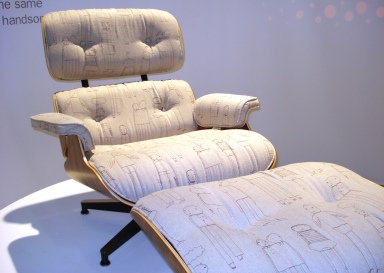
\includegraphics[height=2.25cm]{pics/imagenet-armchairs/armchairs/171272865_de284ebca6.jpg}
\hspace*{0pt}
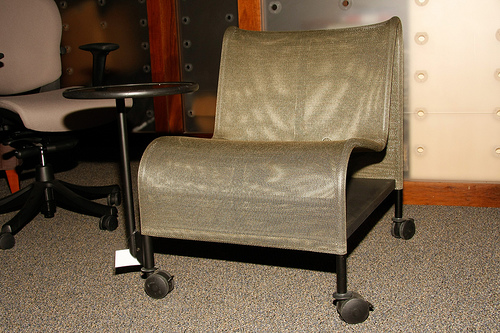
\includegraphics[height=2.25cm]{pics/imagenet-armchairs/armchairs/2244045079_ce65f3f106.jpg}

\vspace*{-8pt}

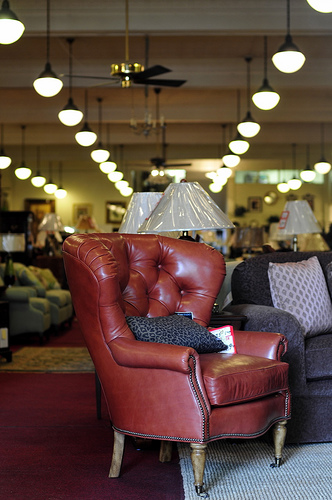
\includegraphics[height=2.25cm]{pics/imagenet-armchairs/armchairs/2463497210_482f74f2bf.jpg}
\hspace*{0pt}
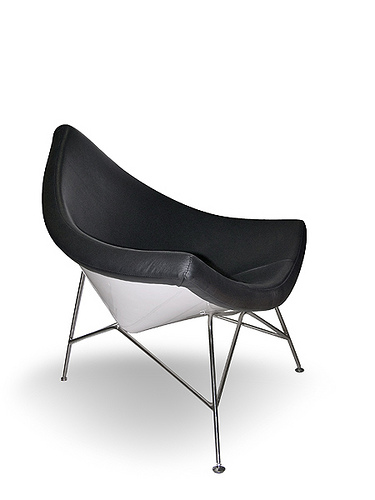
\includegraphics[height=2.25cm]{pics/imagenet-armchairs/armchairs/2114986996_7805c2b63c.jpg}
\hspace*{0pt}
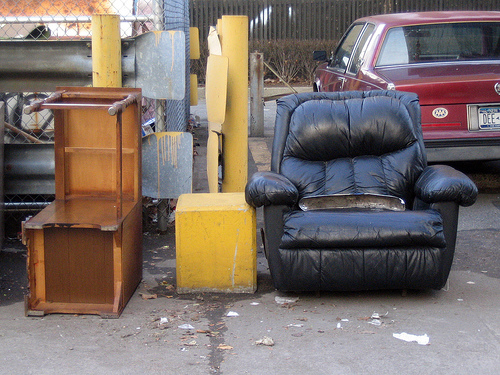
\includegraphics[height=2.25cm]{pics/imagenet-armchairs/armchairs/78510919_04a458def8.jpg}

\acksource{(ImageNet)}

\end{center}

%--------------------------------------------------

\note[2]{

  The core idea of machine learning is to write algorithms that depend
  on parameters whose values are let unspecified, and optimized to
  work on examples.

  When the number of parameters is very large and the type of
  computation carefully chosen, these methods can ``discover'' rich
  and complex processings that would have been impossible to
  handcraft.

  % \vspace*{1em}

  Although there are multiple forms of machine-learning models, most
  of them take as input a real world signal and output a refined
  information: semantic content (object classification), location of
  object (detection), word present in a audio signal (keyword
  spotting), meaning in a sentence (sentiment analysis). Some
  algorithms even take as input a random input to synthesis a
  structured signal: image, sound or text.

  %Why do we need machine learning in general ?

  %% At a more abstract level, it consists of building models from a
  %% finite set of samples, by capturing the statistical regularities of
  %% the world, with a view to making predictions on unseen data, or
  %% generating new signals.

  % \vspace*{1em}

  %% \begin{itemize}
  %% \item Image classification, object detection, image segmentation
  %% \item Sequence classification: sentiment analysis, activity/action
  %% recognition, DNA sequence classification, action selection.
  %% \item Sequence synthesis: text synthesis, music synthesis, motion synthesis.
  %% \item Sequence-to-sequence translation: speech recognition, text
  %% translation, part-of-speech tagging.
  %% \end{itemize}

  % \vspace*{1em}

  The task of automatically extracting the information of interest is
  difficult because of the large variability of the input signal for a
  given task.

  Despite being obvious to the human eye that all the above images
  depict armchairs, it would be very difficult to come up with a
  hand-crafted algorithmic recipe taking as input the image pixels and
  predicting they represent an armchair.

}

\end{frame}

%%%%%%%%%%%%%%%%%%%%%%%%%%%%%%%%%%%%%%%%%%%%%%%%%%%%%%%%%%%%%%%%%%%%%%

\begin{frame}[t] %% frame 2 / 53

\vspace*{2cm}

\mode<beamer>{

\only<1-2>{
%
Our brain is so good at interpreting visual information that the
``semantic gap'' is hard to assess intuitively.
}

\only<2>{
%
\vspace*{-1cm}

\begin{center}
\begin{tikzpicture}
  \draw[draw=none] (-2.5, -2.5) -- (2.5, -2.5) -- (2.5, 2.5) -- (-2.5, 2.5) -- (-2.5 , -2.5);
  \node[inner sep=0pt] (img) at (0.0, 0.0)
       {\raisebox{0.5em}{This:}
         \ \ \ 
\includegraphics[height=0.6cm]{pics/cifar10/cifar_43.png} \ \ \ \ \raisebox{0.5em}{is a horse}};
\end{tikzpicture}
\end{center}
}

\only<3>{
\begin{center}
\begin{tikzpicture}
  \draw[draw=none] (-2.5, -2.5) -- (2.5, -2.5) -- (2.5, 2.5) -- (-2.5, 2.5) -- (-2.5 , -2.5);
  \node[inner sep=0pt,draw=white,thick] (img) at (0.0, 0.0)
       {
\includegraphics[height=4cm]{pics/cifar10/cifar_43.png}};
\end{tikzpicture}
\end{center}
}

\only<4>{
\begin{center}
\begin{tikzpicture}
  \draw[draw=none] (-2.5, -2.5) -- (2.5, -2.5) -- (2.5, 2.5) -- (-2.5, 2.5) -- (-2.5 , -2.5);
  \node[inner sep=0pt,draw=white,thick] (imgB) at (0.25,  0.25)
       {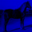
\includegraphics[height=4cm]{pics/cifar10/cifar_43_B.png}};
  \node[inner sep=0pt,draw=white,thick] (imgG) at (0.0,  0.0)
       {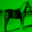
\includegraphics[height=4cm]{pics/cifar10/cifar_43_G.png}};
  \node[inner sep=0pt,draw=white,thick] (imgR) at (-0.25, -0.25)
       {
\includegraphics[height=4cm]{pics/cifar10/cifar_43_R.png}};
\end{tikzpicture}
\end{center}
}
}

\mode<handout>{

\vspace*{-1em}

Our brain\index{brain} is so good at interpreting visual information
that the ``semantic gap''\index{semantic gap} is hard to assess
intuitively.

\vspace*{-1em}

\begin{center}

    \hspace*{\stretch{1}}
    %
    \begin{tikzpicture}[scale=0.5]
      \draw[draw=none] (-2.5, -2.5) -- (2.5, -2.5) -- (2.5, 2.5) -- (-2.5, 2.5) -- (-2.5 , -2.5);
      \node[inner sep=0pt] (img) at (0.0, 0.0)
           {\raisebox{0.5em}{This} \ 
\includegraphics[height=0.6cm]{pics/cifar10/cifar_43.png} \ \ \raisebox{0.5em}{is a horse}};
    \end{tikzpicture}
    %
    \hspace*{\stretch{1}}
    %
    \begin{tikzpicture}[scale=0.5]
      \draw[draw=none] (-2.5, -2.5) -- (2.5, -2.5) -- (2.5, 2.5) -- (-2.5, 2.5) -- (-2.5 , -2.5);
      \node[inner sep=0pt] (img) at (0.0, 0.0)
           {
\includegraphics[height=2cm]{pics/cifar10/cifar_43.png}};
    \end{tikzpicture}
    %
    \hspace*{\stretch{1}}

    \vspace*{-4em}

    \begin{tikzpicture}
      \draw[draw=none] (-2.5, -2.5) -- (2.5, -2.5) -- (2.5, 2.5) -- (-2.5, 2.5) -- (-2.5 , -2.5);
      \node[inner sep=0pt] (imgB) at (0.25,  0.25)
           {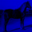
\includegraphics[height=2cm]{pics/cifar10/cifar_43_B.png}};
      \node[inner sep=0pt] (imgG) at (0.0,  0.0)
           {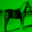
\includegraphics[height=2cm]{pics/cifar10/cifar_43_G.png}};
      \node[inner sep=0pt] (imgR) at (-0.25, -0.25)
           {
\includegraphics[height=2cm]{pics/cifar10/cifar_43_R.png}};
    \end{tikzpicture}


\end{center}

}


%--------------------------------------------------

\note[0]{

  When discussing the subject with people who are not from the field,
  it is intriguing to them that there is so much effort in making
  computers do what humans do so easily. Very often people do not
  realize that the problem actually exists.

  % \vspace*{1em}

  The semantic gap is the difference there exists between a raw signal
  and its semantic content. For instance, two images can be very
  different in terms of pixel values, although depicting the same
  object. While it is even hard to be aware of the processing
  happening in our visual cortex when we look at an image such as the
  small vignette of a horse above, the larger pixelated image is
  slightly more difficult to parse since edges along the animal are
  not apparent anymore, while artificial pixel edges are. When the
  image is split into its three color component red/green/blue, that
  correspond to the representation in memory, our visual system has
  greater difficulty to understand the signal.

}

\end{frame}

%%%%%%%%%%%%%%%%%%%%%%%%%%%%%%%%%%%%%%%%%%%%%%%%%%%%%%%%%%%%%%%%%%%%%%

\begin{frame}[fragile]

\begin{comment}
from torchvision.datasets import CIFAR10
cifar = CIFAR10('./data/cifar10/', train=True, download=True)
x = torch.from_numpy(cifar.data)[43].permute(2, 0, 1)
x[:, :4, :8]
\end{comment}

\begin{rawsrc}
>>> from torchvision.datasets import CIFAR10
>>> cifar = CIFAR10('./data/cifar10/', train=True, download=True)
Files already downloaded and verified
>>> x = torch.from_numpy(cifar.data)[43].permute(2, 0, 1)
>>> x[:, :4, :8]
tensor([[[ 99,  98, 100, 103, 105, 107, 108, 110],
         [100, 100, 102, 105, 107, 109, 110, 112],
         [104, 104, 106, 109, 111, 112, 114, 116],
         [109, 109, 111, 113, 116, 117, 118, 120]],

        [[166, 165, 167, 169, 171, 172, 173, 175],
         [166, 164, 167, 169, 169, 171, 172, 174],
         [169, 167, 170, 171, 171, 173, 174, 176],
         [170, 169, 172, 173, 175, 176, 177, 178]],

        [[198, 196, 199, 200, 200, 202, 203, 204],
         [195, 194, 197, 197, 197, 199, 200, 201],
         [197, 195, 198, 198, 198, 199, 201, 202],
         [197, 196, 199, 198, 198, 199, 200, 201]]], dtype=torch.uint8)
\end{rawsrc}

%--------------------------------------------------

\note[0]{

  In the memory of the computer, images are stored as tensors, which
  are multi-dimensional data structures storing the pixel values.

  Tensors are truly what algorithms have access to operate on and
  solve the task they are trained for.

  So an ``image recognition'' algorithms should predict that there is
  a horse in the input image from this table of integers.

}

\end{frame}

%%%%%%%%%%%%%%%%%%%%%%%%%%%%%%%%%%%%%%%%%%%%%%%%%%%%%%%%%%%%%%%%%%%%%%

\begin{frame} %% frame 4 / 53

Extracting semantic\index{semantic} automatically requires models of
extreme complexity, which cannot be designed by hand.

Techniques used in practice consist of
\begin{enumerate}
\item defining a parametric model\index{parametric model}, and
\item optimizing\index{optimization} its parameters by ``making it
work'' on training data.
\end{enumerate}

\pause

This is similar to biological\index{biology} systems for which the
model ({e.g.} brain structure\index{brain}) is DNA-encoded, and
parameters ({e.g.} synaptic weights\index{synaptic weights}) are
tuned through experiences.

\pause

%% \vspace*{\stretch{1}}

Deep learning encompasses software technologies to scale-up to
billions of model parameters and as many training examples.

%--------------------------------------------------

\note[0]{%
  %
  In some very controlled environments such as in an automatic factory
  assembly line, it may sometimes be possible to design models by
  hand, but in most real-world vision problems images are prone to
  many variations due to illumination, geometric pose, occlusion,
  texture, articulated bodies, {etc.} which makes it impossible to
  design a model by hand to extract their semantic content.

  The standard way of addressing the task of extracting a ``refined''
  information from a high dimensional input signal consists of
  designing an algorithm with a lot of free parameters, that is known,
  for theoretical reasons, or by experience to compute the proper
  responses for adequate values of the parameters. These values are
  then optimized by a procedure on available training examples.

  This process of designing a system whose parameters are changed to
  make it better at a task shares similarities with biological nervous
  systems, whose structure is fixed (DNA-encoded), but whose
  processing is modulated by quantities (synaptic weights) that are
  tuned through experiences.

}

\end{frame}

%%%%%%%%%%%%%%%%%%%%%%%%%%%%%%%%%%%%%%%%%%%%%%%%%%%%%%%%%%%%%%%%%%%%%%

\begin{frame}{}{} %% frame 5 / 53

There are strong connections between standard statistical modeling and
machine learning.

\pause

Classical ML\index{shallow learning} methods combine a ``learnable''
model from statistics ({e.g.} ``linear regression''\index{linear
  regression}) with prior knowledge in pre-processing.

\pause

``Artificial neural networks'' pre-dated these approaches, and do not
follow this dichotomy. They consist of ``deep'' stacks of
parametrized processing.

%--------------------------------------------------

\note[2]{

  Most of standard statistical methods ({e.g.} logistic
  regression, linear regression) do not allow to deal with signals of
  very high dimensions such as images.

  Therefore, we usually combine them with a hand designed
  pre-processing step which extracts a small number of meaningful
  quantities from the raw signal. Hopefully, this pre-processing step
  retains all the information content useful to make the prediction.

  Classical machine learning methods follow this dichotomy of
  %
  \begin{itemize}

  \item first, processing the signal to extract features in a ad-hoc
    manner,

  \item second, feeding these features to a statistical processing
    that makes a prediction, and can be tuned to work on training
    examples.

  \end{itemize}
  %
  as opposed to artificial neural networks, which are series of
  parametrized processing units, each of them extracting meaningful
  values and making predictions at the same time.

  The term ``deep'' in ``deep learning'' refers to the fact that many
  of these modules are stacked together.

}


\end{frame}

%%%%%%%%%%%%%%%%%%%%%%%%%%%%%%%%%%%%%%%%%%%%%%%%%%%%%%%%%%%%%%%%%%%%%%

\sectiontitleframe{From artificial neural networks to ``Deep Learning''}

%% https://en.wikibooks.org/wiki/Artificial_Neural_Networks/History

%% In 1949, Donald Hebb published The Organization of Behavior, which
%% outlined a law for synaptic neuron learning. This law, later known as
%% Hebbian Learning in honor of Donald Hebb is one of the simplest and
%% most straight-forward learning rules for artificial neural networks.

%% In 1951, Marvin Minsky created the first ANN while working at
%% Princeton.

%% In 1958 The Computer and the Brain was published posthumously, a year
%% after John von Neumann’s death. In that book, von Neumann proposed
%% many radical changes to the way in which researchers had been modeling
%% the brain.

%% The Mark I Perceptron was also created in 1958, at Cornell University
%% by Frank Rosenblatt. The Perceptron was an attempt to use neural
%% network techniques for character recognition. The Mark I Perceptron
%% was a linear system, and was useful for solving problems where the
%% input classes were linearly separable in the input space. In 1960,
%% Rosenblatt published the book Principles of Neurodynamics, containing
%% much of his research and ideas about modeling the brain.

%% The backpropagation algorithm, originally discovered by Werbos in 1974
%% was rediscovered in 1986 with the book Learning Internal
%% Representation by Error Propagation by Rumelhart, Hinton and
%% Williams. Backpropagation is a form of the gradient descent algorithm
%% used with artificial neural networks for minimization and
%% curve-fitting.

%%%%%%%%%%%%%%%%%%%%%%%%%%%%%%%%%%%%%%%%%%%%%%%%%%%%%%%%%%%%%%%%%%%%%%

\begin{frame}{}{} %% frame 6 / 53

\begin{center}

Networks of ``Threshold Logic Unit''

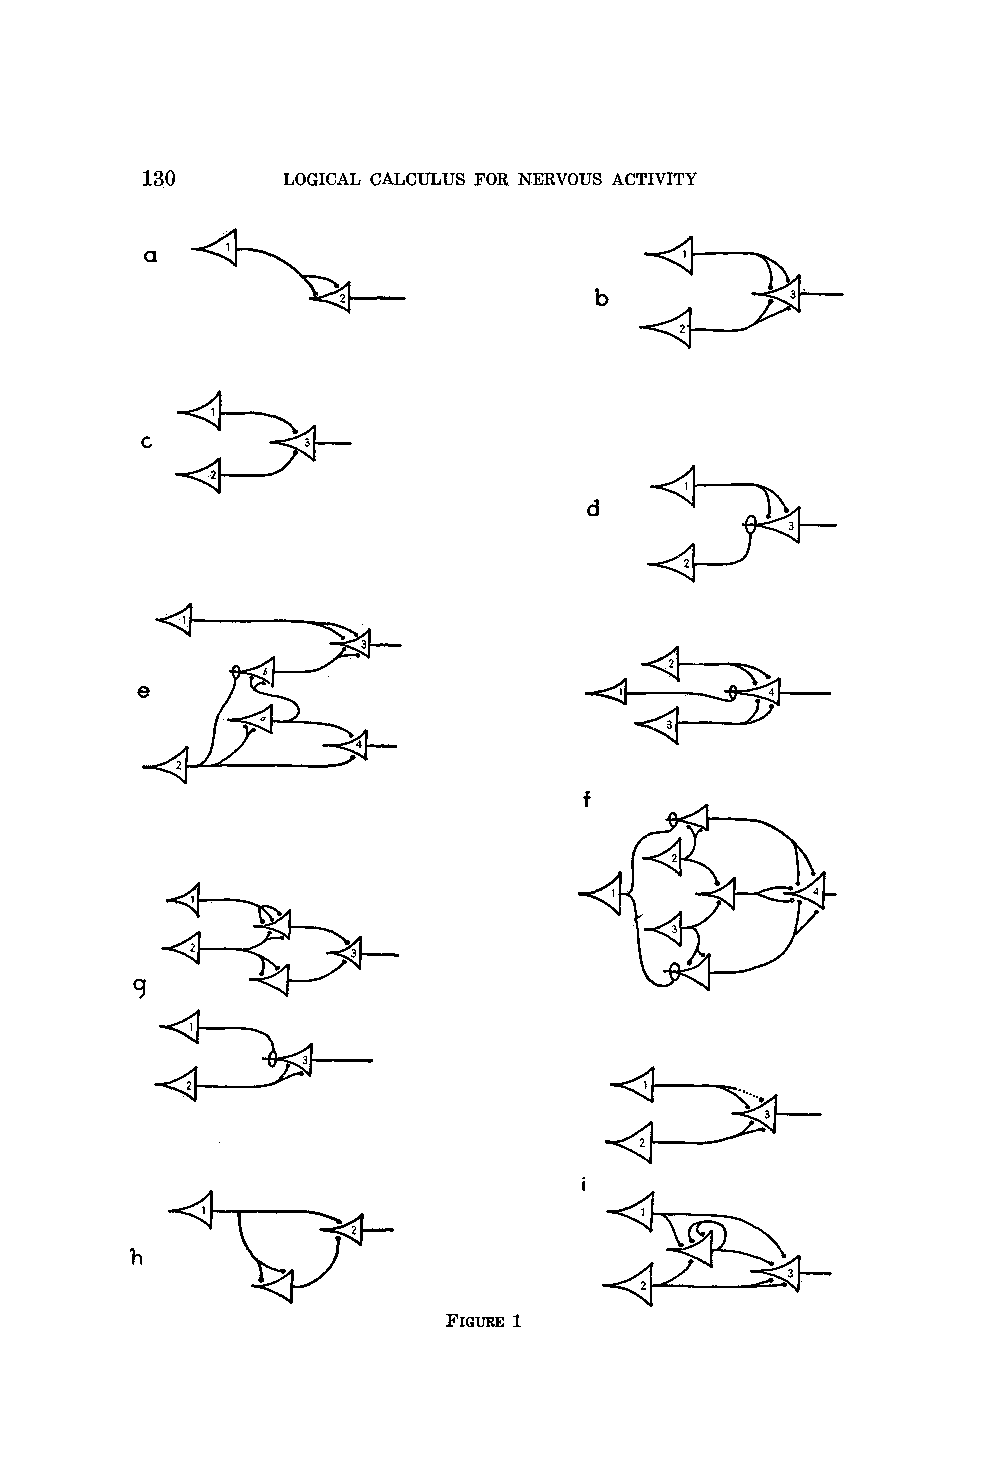
\includegraphics[clip,trim=60 73 60 95,scale=0.30] {excerpts/mcculloch_pitts_1943_page_16.pdf}

\acksource{\citep{McCulloch1943}}

\end{center}

%--------------------------------------------------

\note[0]{

  We can trace back the origins of neural networks to
  \cite{McCulloch1943} who proposed to model the nervous system as a
  network of ``threshold logic units.'' They suggested that one can
  put all the intelligence in the connections: elementary units doing
  very simple computation can perform an arbitrary mathematical
  function by being combined in an appropriate manner.

  This opened the way to the notion that one can have a class of
  processing methods which are parameterized through the connections
  between units.

}

\end{frame}

%%%%%%%%%%%%%%%%%%%%%%%%%%%%%%%%%%%%%%%%%%%%%%%%%%%%%%%%%%%%%%%%%%%%%%

\begin{frame}{}{} %% frame 7 / 53

%% \includegraphics[clip,trim=25 220 40 66,scale=0.25] {./excerpts/hubel_wiesel_1962_p26.pdf} \\[1em]

%% \acksource{\citep{hubel1962receptive}}

\vspace*{-4ex}

\begin{center}
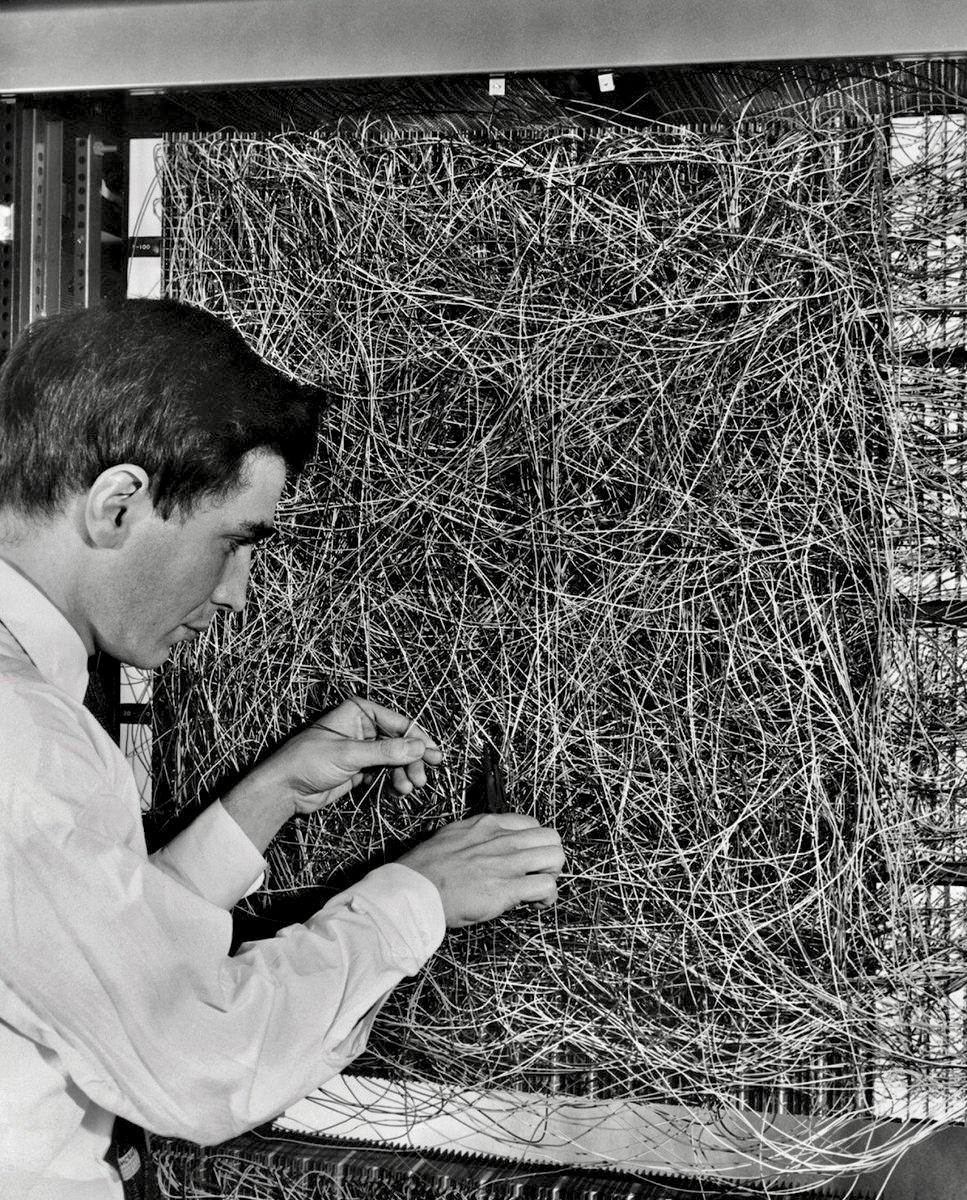
\includegraphics[height=3.5cm]{pics/Rosenblatt_Mark_I_perceptron_1956.jpg}

Frank Rosenblatt working on the Mark I perceptron (1956)
\end{center}

\vspace*{2ex}

\begin{itemize}
\item<1->[1949 --] Donald Hebb proposes the Hebbian Learning principle
  \citep{hebb-organization-of-behavior-1949}.
\item<1->[1951 --] Marvin Minsky creates the first ANN (Hebbian learning, 40 neurons).
\item<2->[1958 --] Frank Rosenblatt creates a perceptron to classify $20 \times 20$
  images.
\item<3->[1959 --] David H. Hubel and Torsten Wiesel demonstrate
  orientation selectivity and columnar organization in the cat's
  visual cortex \citep{hubel1962receptive}.
%% \item[1974 --] Paul Werbos proposes the back-propagation.
\item<4->[1982 --] Paul Werbos proposes back-propagation for ANNs \citep{Werbos1981}.
\end{itemize}

%--------------------------------------------------

\note[0]{

  The Hebbian Learning principle is a simple rule that allows to learn
  patterns and decision rules by reinforcing the connections between
  neurons when they tend to activate simultaneously. Although
  biologically plausible it is not used nowadays in machine learning.

  A perceptron is the simplest form of neural network, composed of a
  single neuron.

  Hubel and Wiesel's studies of the visual cortex of a cat showed that
  the visual information goes through a series of several processing
  steps: edge detections, combination of edges, detection of motion of
  edges, {etc.} These results built a strong bridge between the neural
  processing and the mathematical world, in particular signal
  processing.

  The key component of deep learning is the back-propagation algorithm
  which was proposed by Werbos. Back-propagation is used to train
  neural networks and is a straight-forward application of the chain
  rule from differential calculus.

}

\end{frame}

%% In a 1958 press conference organized by the US Navy, Rosenblatt made
%% statements about the perceptron that caused a heated controversy among
%% the fledgling AI community; based on Rosenblatt's statements, The New
%% York Times reported the perceptron to be "the embryo of an electronic
%% computer that [the Navy] expects will be able to walk, talk, see,
%% write, reproduce itself and be conscious of its existence."

%%%%%%%%%%%%%%%%%%%%%%%%%%%

\begin{frame}{}{} %% frame 8 / 53

\label{thumbnail-slide}

\begin{center}

Neocognitron\index{neocognitron}

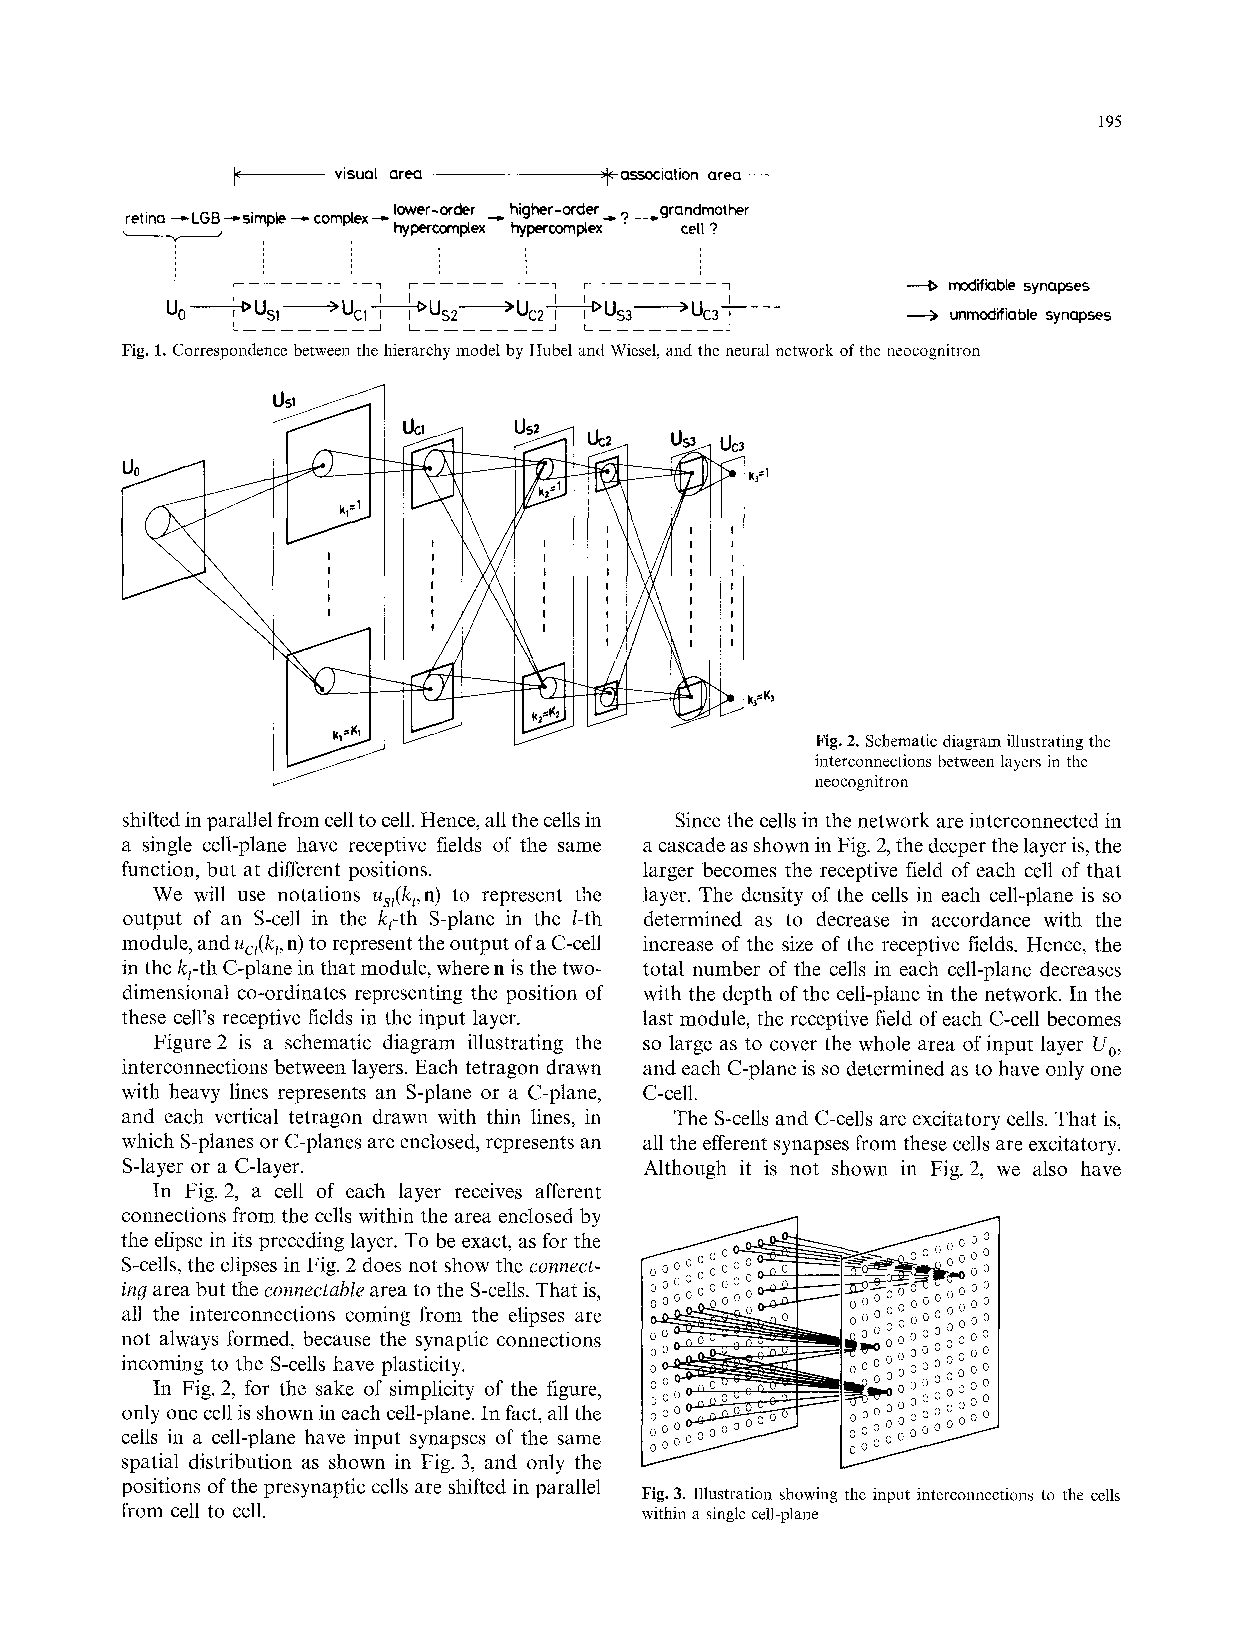
\includegraphics[clip,trim=50 405 220 175,scale=0.7] {excerpts/fukushima_1980_page_3.pdf}

\acksource{\citep{Fukushima1980Neocognitron}}

This model follows Hubel and Wiesel's results.

\end{center}

%--------------------------------------------------

\note[0]{

  \cite{Fukushima1980Neocognitron} implemented the results of Hubel
  and Wiesel in a model called the Neocognitron. It was used for
  handwritten character recognition and can be viewed as the precursor
  of modern convolution networks.

}

\end{frame}

%%%%%%%%%%%%%%%%%%%%%%%%%%%%%%%%%%%%%%%%%%%%%%%%%%%%%%%%%%%%%%%%%%%%%%

\begin{frame}{}{} %% frame 9 / 53

\begin{center}

Network for the T-C problem

\hspace*{1cm}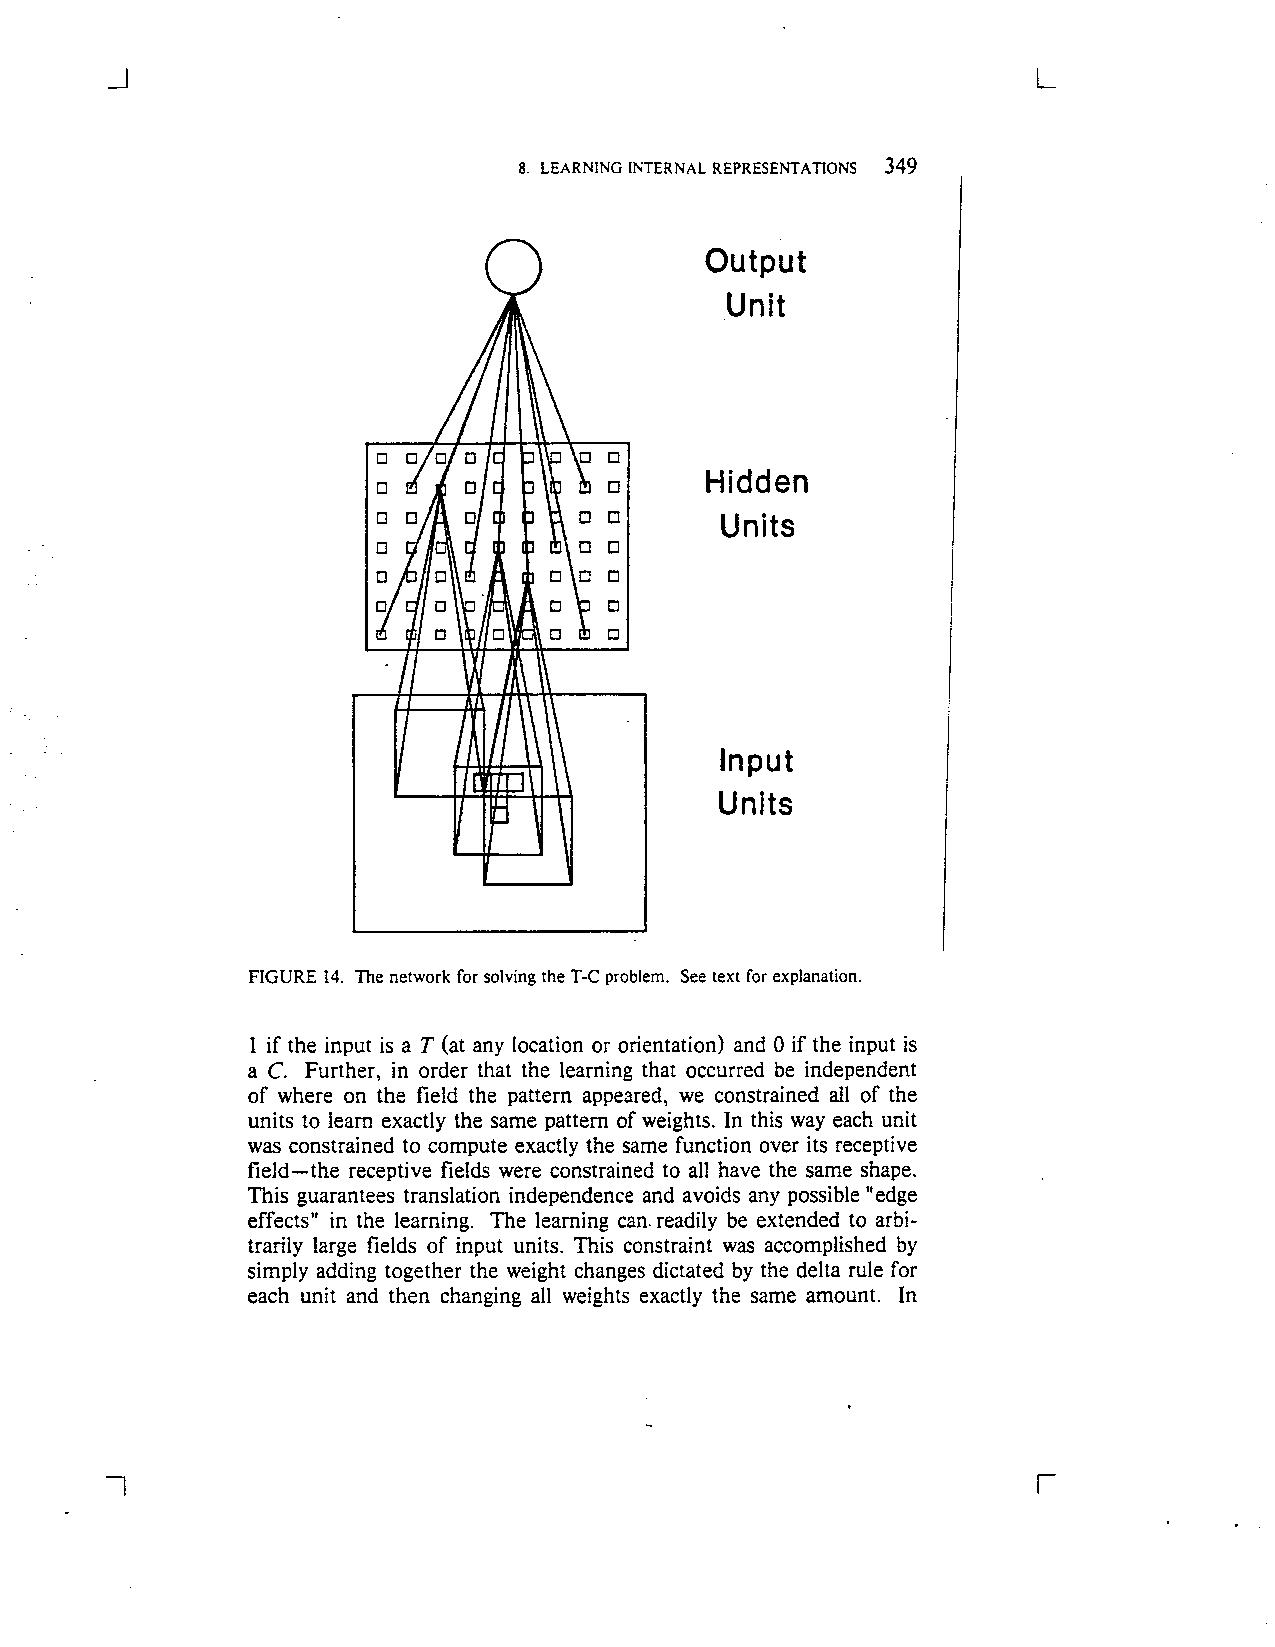
\includegraphics[clip,trim=160 335 210 110,scale=0.5] {excerpts/rumelhart_et_al_1986_page_32.pdf}

Trained with back-prop.

\acksource{\citep{Rumelhart1986book}}
\end{center}

%--------------------------------------------------

\note[0]{

  \cite{Rumelhart1986book} used back-propagation to train a network
  similar to the Neocognitron, and showed that the so-called
  ``hidden'' units, which are neither input nor output neurons, learn
  meaningful representation of the data.

}

\end{frame}

%%%%%%%%%%%%%%%%%%%%%%%%%%%%%%%%%%%%%%%%%%%%%%%%%%%%%%%%%%%%%%%%%%%%%%

\begin{frame}{}{}

\begin{center}

LeNet family\index{LeNet}

%% \vspace*{5mm}

%% \fbox{
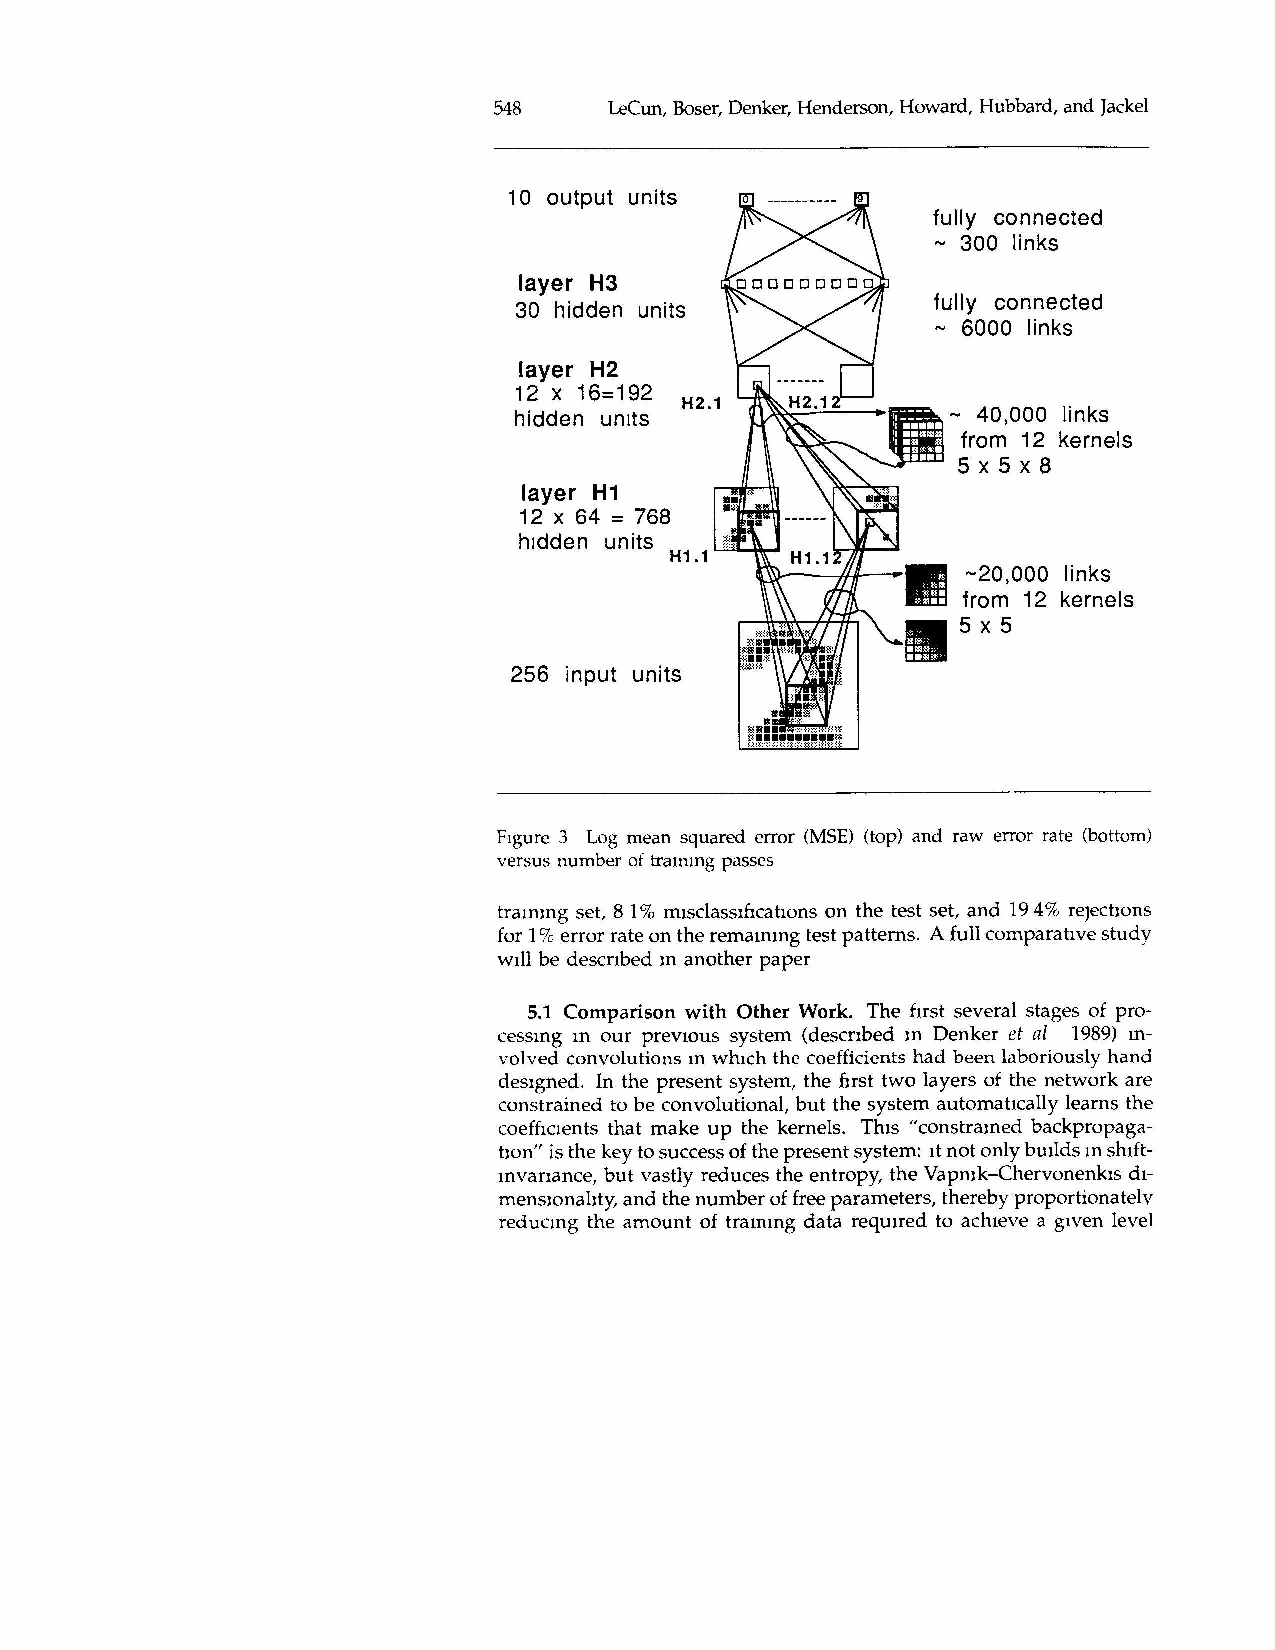
\includegraphics[clip,trim=240 425 50 80,scale=0.65] {excerpts/lecun89_08.pdf}
%% }

\vspace*{-5mm}

\acksource{\citep{lecun1989}}

\end{center}

%--------------------------------------------------

\note[0]{

  \cite{lecun1989} proposed a convolution neural network (CNN, or
  ``convnet'') very similar to modern architectures used nowadays.

  As we shall see later on, a convnet is a series of ``layers'' which
  compute at every location of their input matching scores with small
  templates, and propagate the said matching scores to the next
  layer. These templates are optimized with variants of the
  back-propagation algorithm.

}

\end{frame}

%%%%%%%%%%%%%%%%%%%%%%%%%%%%%%%%%%%%%%%%%%%%%%%%%%%%%%%%%%%%%%%%%%%%%%

%% \begin{frame}{}{} %% frame 10 / 53

%% \begin{center}

%% LeNet-5

%% \vspace*{5mm}

%% \includegraphics[clip,trim=40 590 40 50,scale=0.575] {excerpts/lecun1998_page_7.pdf}

%% \acksource{\citep{lecun1998}}

%% \end{center}

%% \end{frame}

%%%%%%%%%%%%%%%%%%%%%%%%%%%%%%%%%%%%%%%%%%%%%%%%%%%%%%%%%%%%%%%%%%%%%%

\begin{frame}{}{} %% frame 17 / 53

ImageNet\index{ImageNet} Large Scale Visual Recognition
Challenge\index{ILSVRC}.

%% \acksource{\citep{ILSVRC15}}

\vspace*{-1em}

\begin{center}

Started 2010, 1 million images, 1000 categories

\vspace*{-2ex}

\mode<beamer>{

%% \only<+>{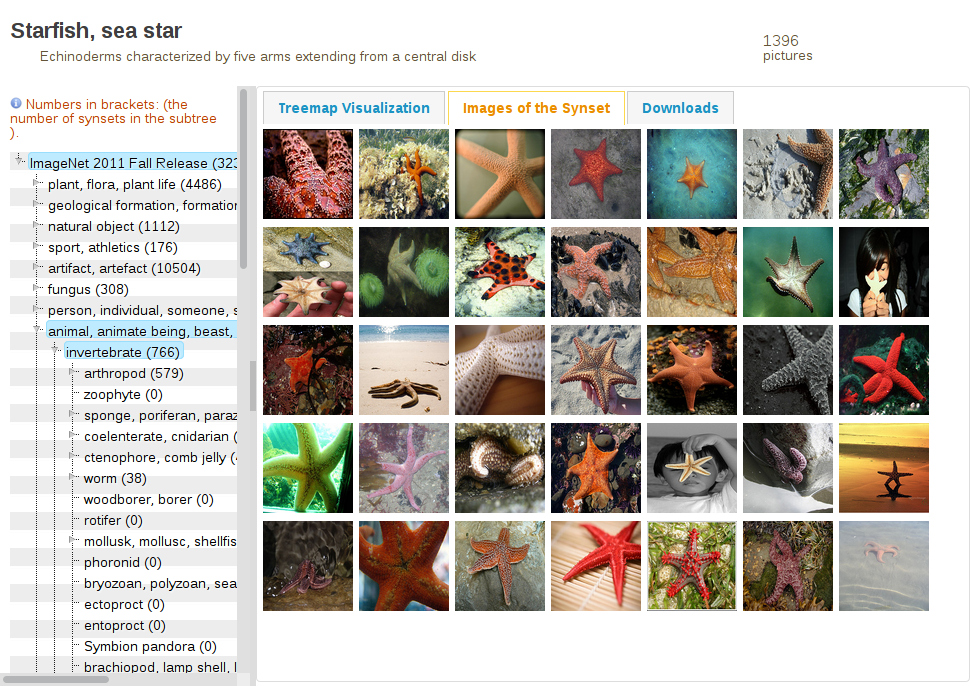
\includegraphics[scale=0.25]{pics/imagenet2012/imagenet2012_starfish.png}}

%% \only<+>{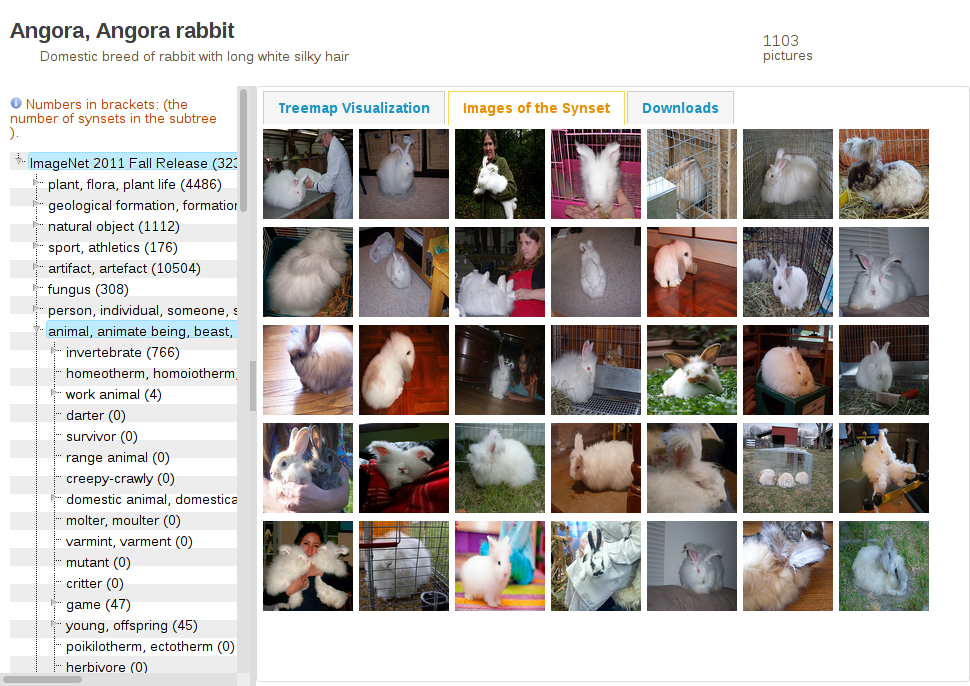
\includegraphics[scale=0.25]{pics/imagenet2012/imagenet2012_angora-rabbit.png}}

%% \only<+>{\includegraphics[scale=0.25]{pics/imagenet2012/imagenet2012_hippopotamus.png}}

%% \only<+>{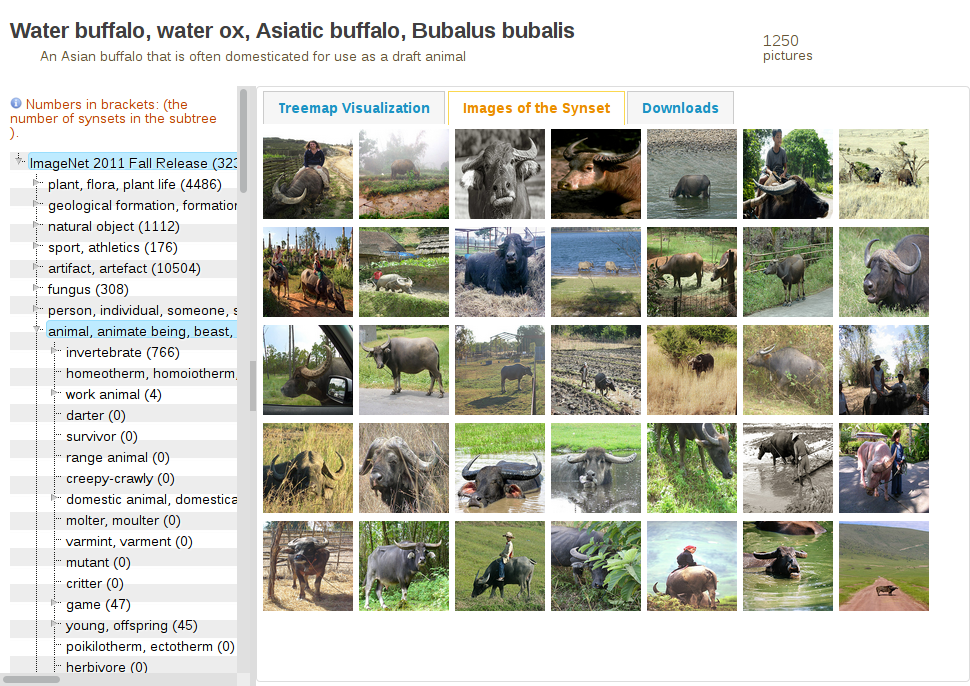
\includegraphics[scale=0.25]{pics/imagenet2012/imagenet2012_water-buffalo.png}}

\only<+>{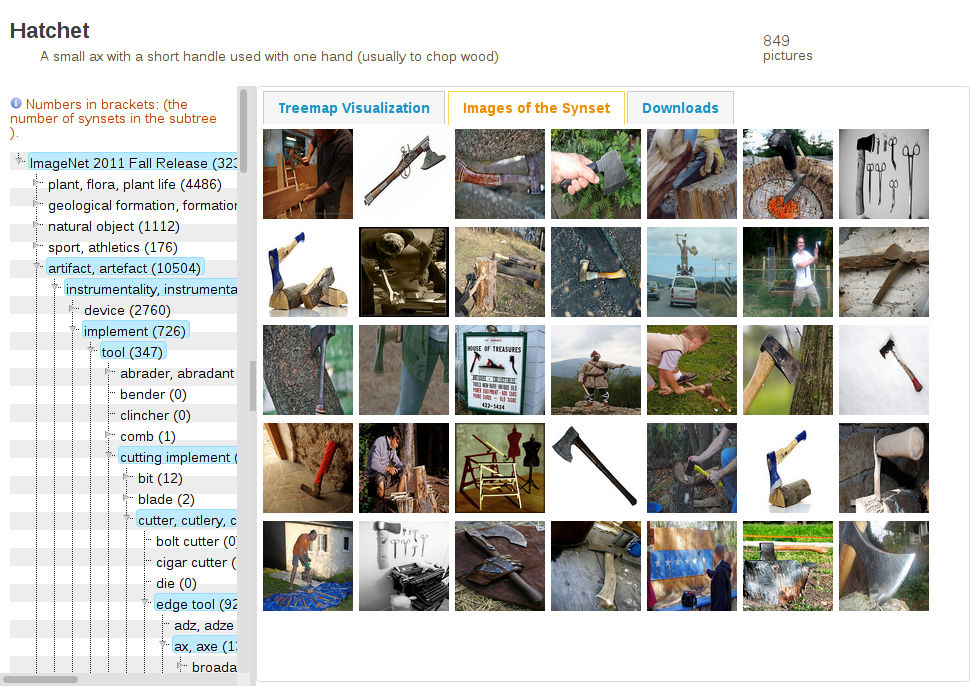
\includegraphics[scale=0.25]{pics/imagenet2012/imagenet2012_hatchet.png}}

}

\mode<handout>{

\hspace*{\stretch{1}}
%
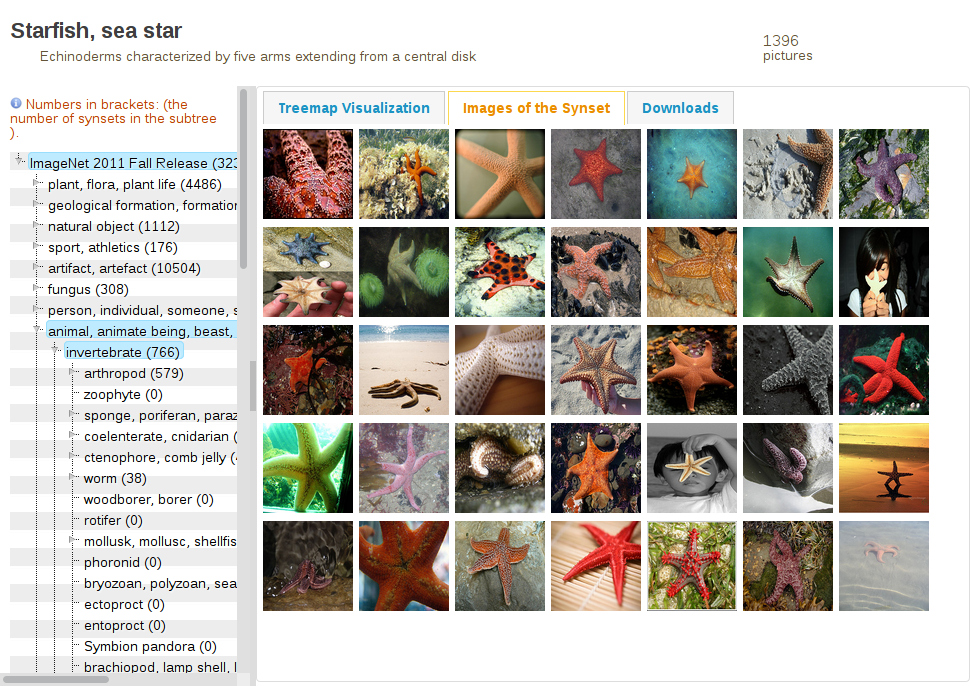
\includegraphics[scale=0.1]{pics/imagenet2012/imagenet2012_starfish.png}
%
\hspace*{\stretch{1}}
%
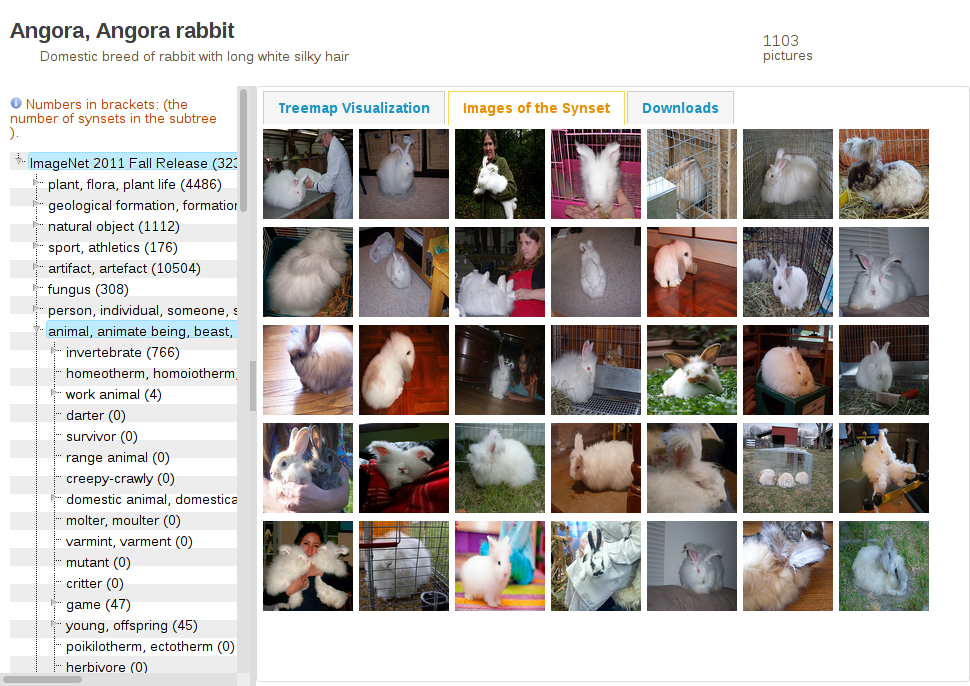
\includegraphics[scale=0.1]{pics/imagenet2012/imagenet2012_angora-rabbit.png}
%
\hspace*{\stretch{1}}

%
%\includegraphics[scale=0.1]{pics/imagenet2012/imagenet2012_hippopotamus.png}

\hspace*{\stretch{1}}
%
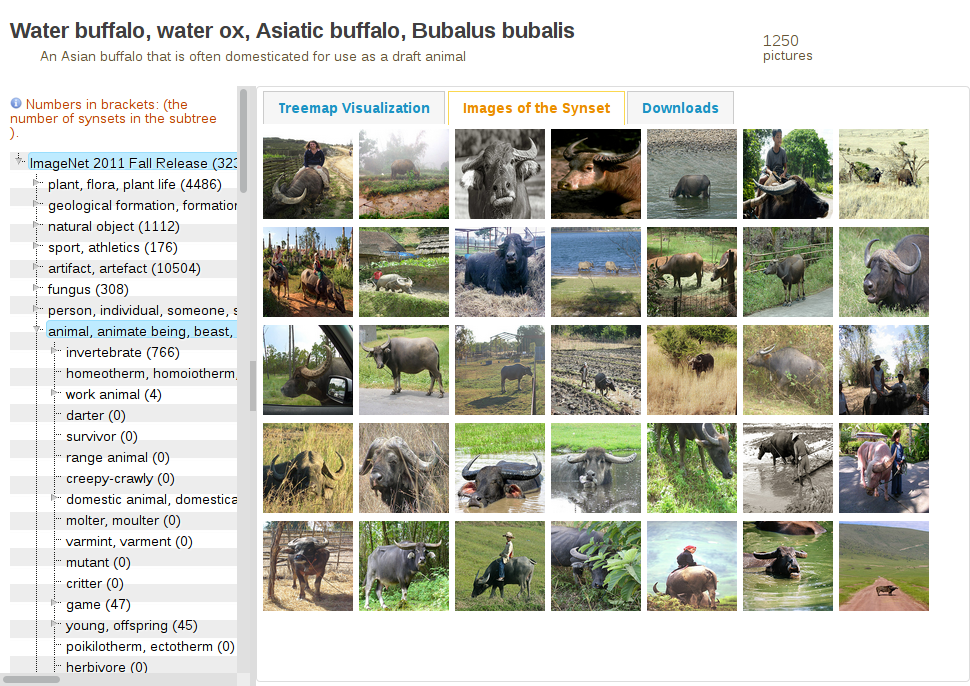
\includegraphics[scale=0.1]{pics/imagenet2012/imagenet2012_water-buffalo.png}
%
\hspace*{\stretch{1}}
%
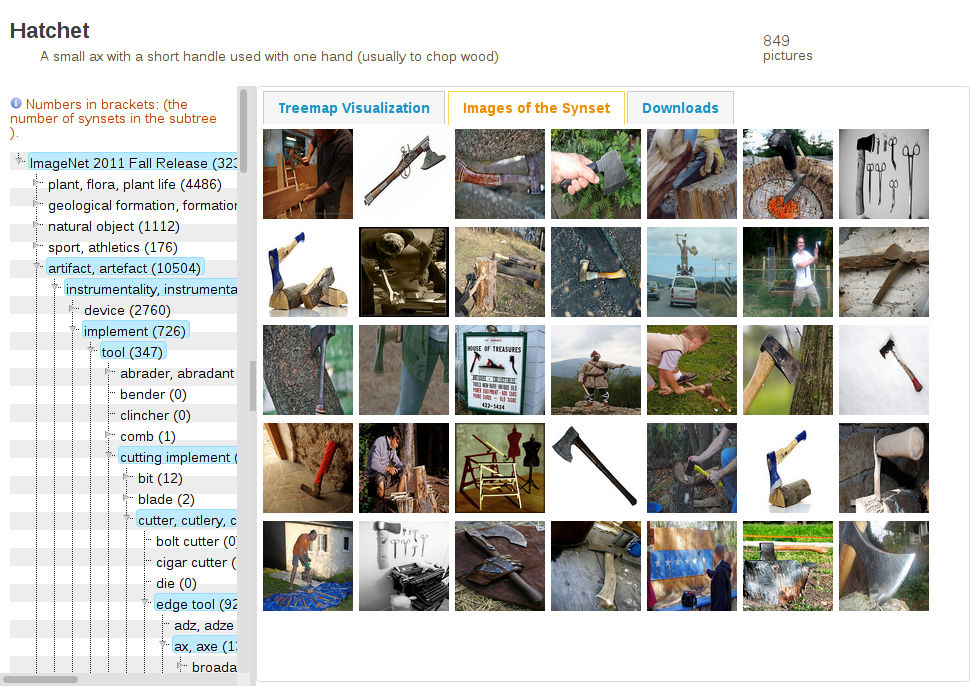
\includegraphics[scale=0.1]{pics/imagenet2012/imagenet2012_hatchet.png}
%
\hspace*{\stretch{1}}

}

\end{center}

\vspace*{-1em}

\acksource{(http://image-net.org/challenges/LSVRC/2014/browse-synsets)}

%--------------------------------------------------

\note[2]{

  The availability of large amount of training data is critical to the
  success of deep-learning methods. ImageNet was started precisely to
  fullfill the need of machine learning, and the subset used to
  benchmark models is composed of more than a million of images
  organized in 1000 categories as diverse as ``angora rabbit'',
  ``German shepherd'', ``acoustic guitar'', or ``school bus''.

  ImageNet was key in the development of deep learning because it
  is of the size required to train deep architectures.

  Most image classification models are trained on this dataset, which
  is split in three parts: the training set, the validation (or dev)
  set, and the test set. The overall goal is to train a model on the
  training data, tune the hyper-parameters on the validation set, and
  finally evaluate the performance of the final model on the test set.

  The testing part consists in:
  %
  \begin{itemize}
  \item applying the model on each test image: the model returns a
  value between 0 and 999, corresponding to the class the model
  believes the image belongs to;
  \item then counting how many times the prediction of the model is
  right.
  \end{itemize}

  There are variants as well, such as the top-5 error rate, which is
  considering the prediction correct if the correct class is among the
  5 first classes predicted by the network.

  It is also common practice for many computer vision tasks, to start
  from a network that was trained on ImageNet, and to refine its
  training on another task and/or extend it.

}

\end{frame}

%%%%%%%%%%%%%%%%%%%%%%%%%%%%%%%%%%%%%%%%%%%%%%%%%%%%%%%%%%%%%%%%%%%%%%

\begin{frame}{}{} %% frame 11 / 53

\begin{center}

AlexNet\index{AlexNet}

\vspace*{5mm}

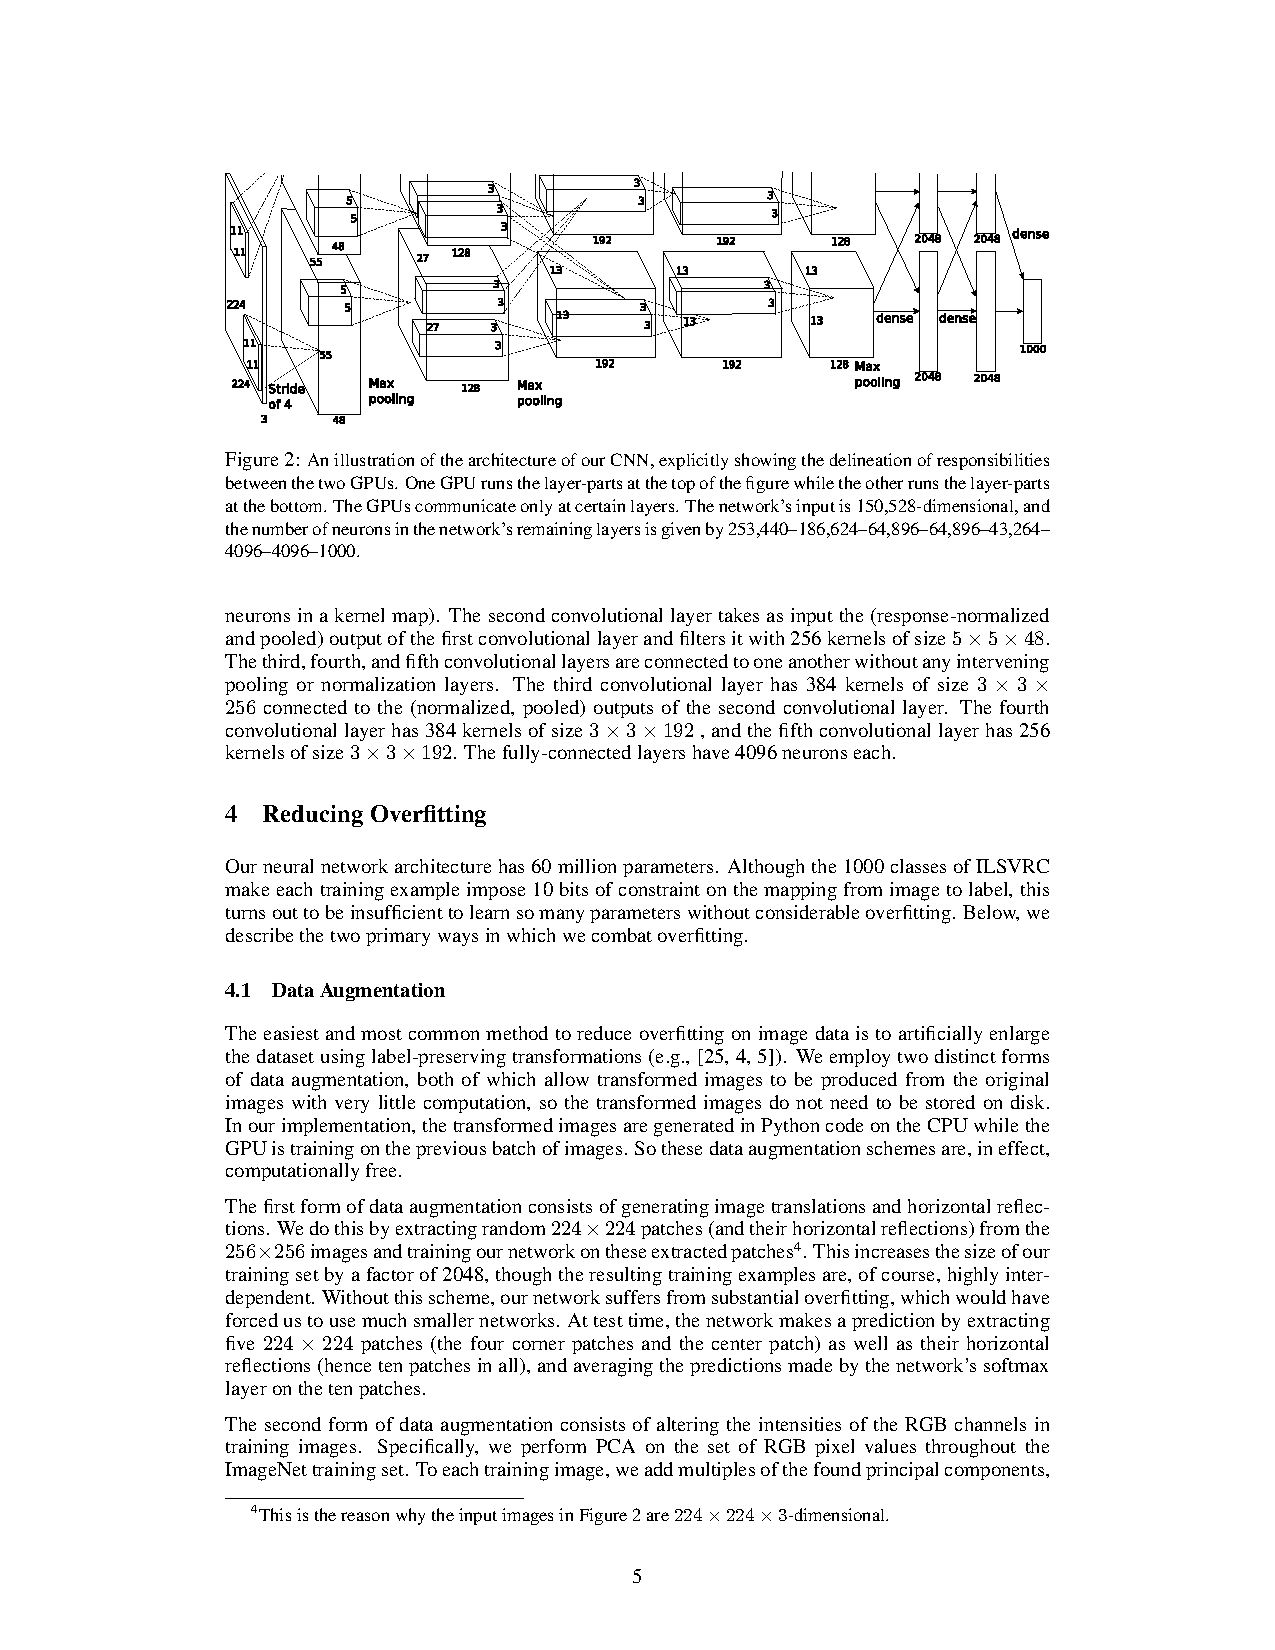
\includegraphics[clip,trim=100 580 100 80,scale=0.7] {excerpts/krizhevsky_2012_page_5.pdf}

\vspace*{-0.25cm}

\acksource{\citep{alexnet2012}}

\end{center}

%--------------------------------------------------

\note[0]{

  Following some earlier work from \cite{ciresan2011}, the work of
  \cite{alexnet2012} showed that a network very similar to a LeNet5,
  but of far greater size, implemented on a graphical card could beat
  by a large margin state-of-the-art image classification methods on
  what was the reference benchmark of the community.

  This work opened the way of training bigger networks on GPUs and
  started a new era of artificial neural networks.

}

\end{frame}

%%%%%%%%%%%%%%%%%%%%%%%%%%%%%%%%%%%%%%%%%%%%%%%%%%%%%%%%%%%%%%%%%%%%%%

\begin{frame}{}{}

%% \vspace*{3ex}

\begin{center}

Top-5 error rate on ImageNet

%ff% \includegraphics[height=7.5cm]{pics/performance_imagenet_2010_2017.png}
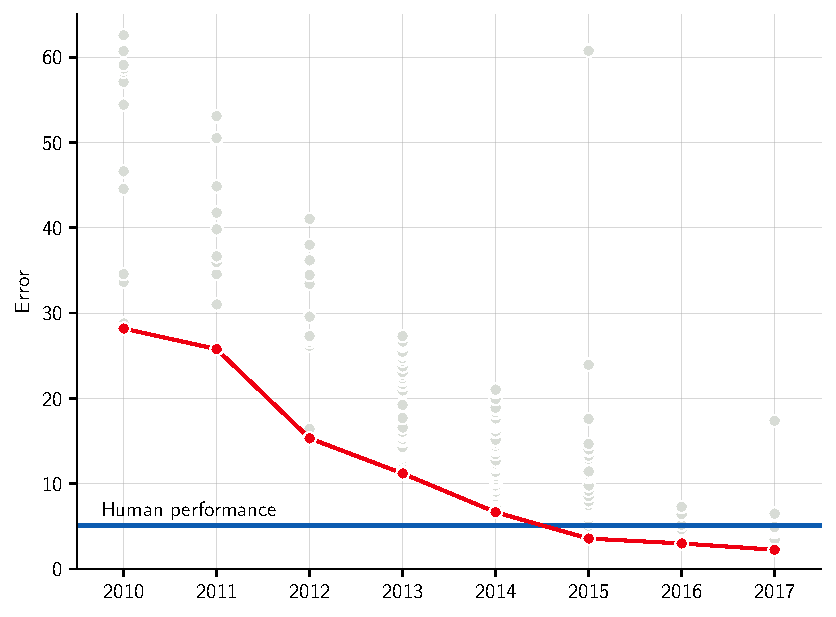
\includegraphics[height=7cm]{materials/imagenet/pics/slides/imagenet.pdf}
%oc% \scalebox{0.65}{\input{materials/imagenet/pics/slides/imagenet.pgf}}

\index{ImageNet}\index{ILSVRC}

\end{center}

\vspace*{-4ex}

\acksource{\citep{gershgorn2017}}

%--------------------------------------------------

\note[0]{

  Each gray dot on this graph shows the error rate of a model. The red
  line indicates the state-of-the-art performance each year, and the
  blue line shows the performance of humans asked to make the
  prediction, which can be seen as a gold standard.

  A model may outperform humans if it picks statistical regularities
  that humans do not perceive, probably because of a bias in the data
  set.

}

\end{frame}

%%%%%%%%%%%%%%%%%%%%%%%%%%%%%%%%%%%%%%%%%%%%%%%%%%%%%%%%%%%%%%%%%%%%%%

\begin{frame}{}{} %% frame 12 / 53

\begin{tabular}{cp{1cm}c}
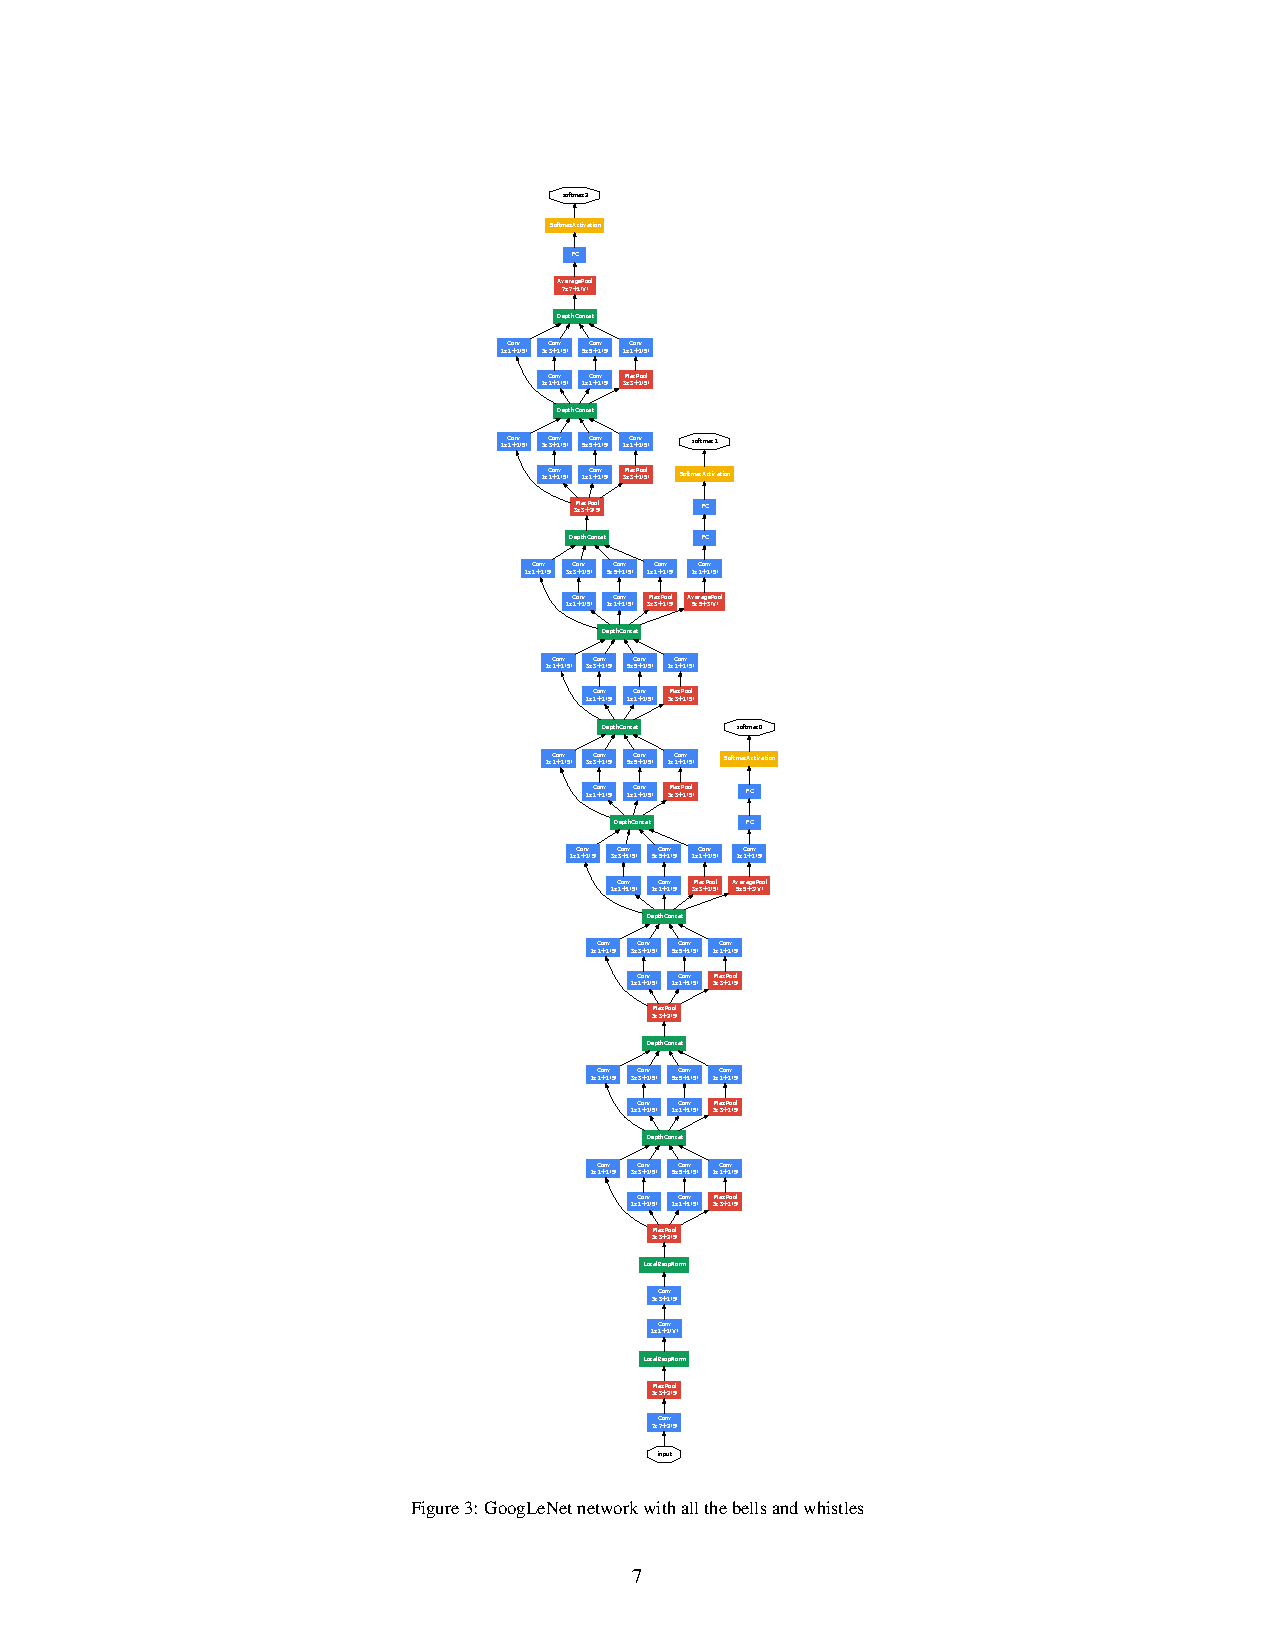
\includegraphics[clip,trim=230 80 220 80,scale=0.3]{excerpts/szegedy_2014_page_7.pdf}
&&
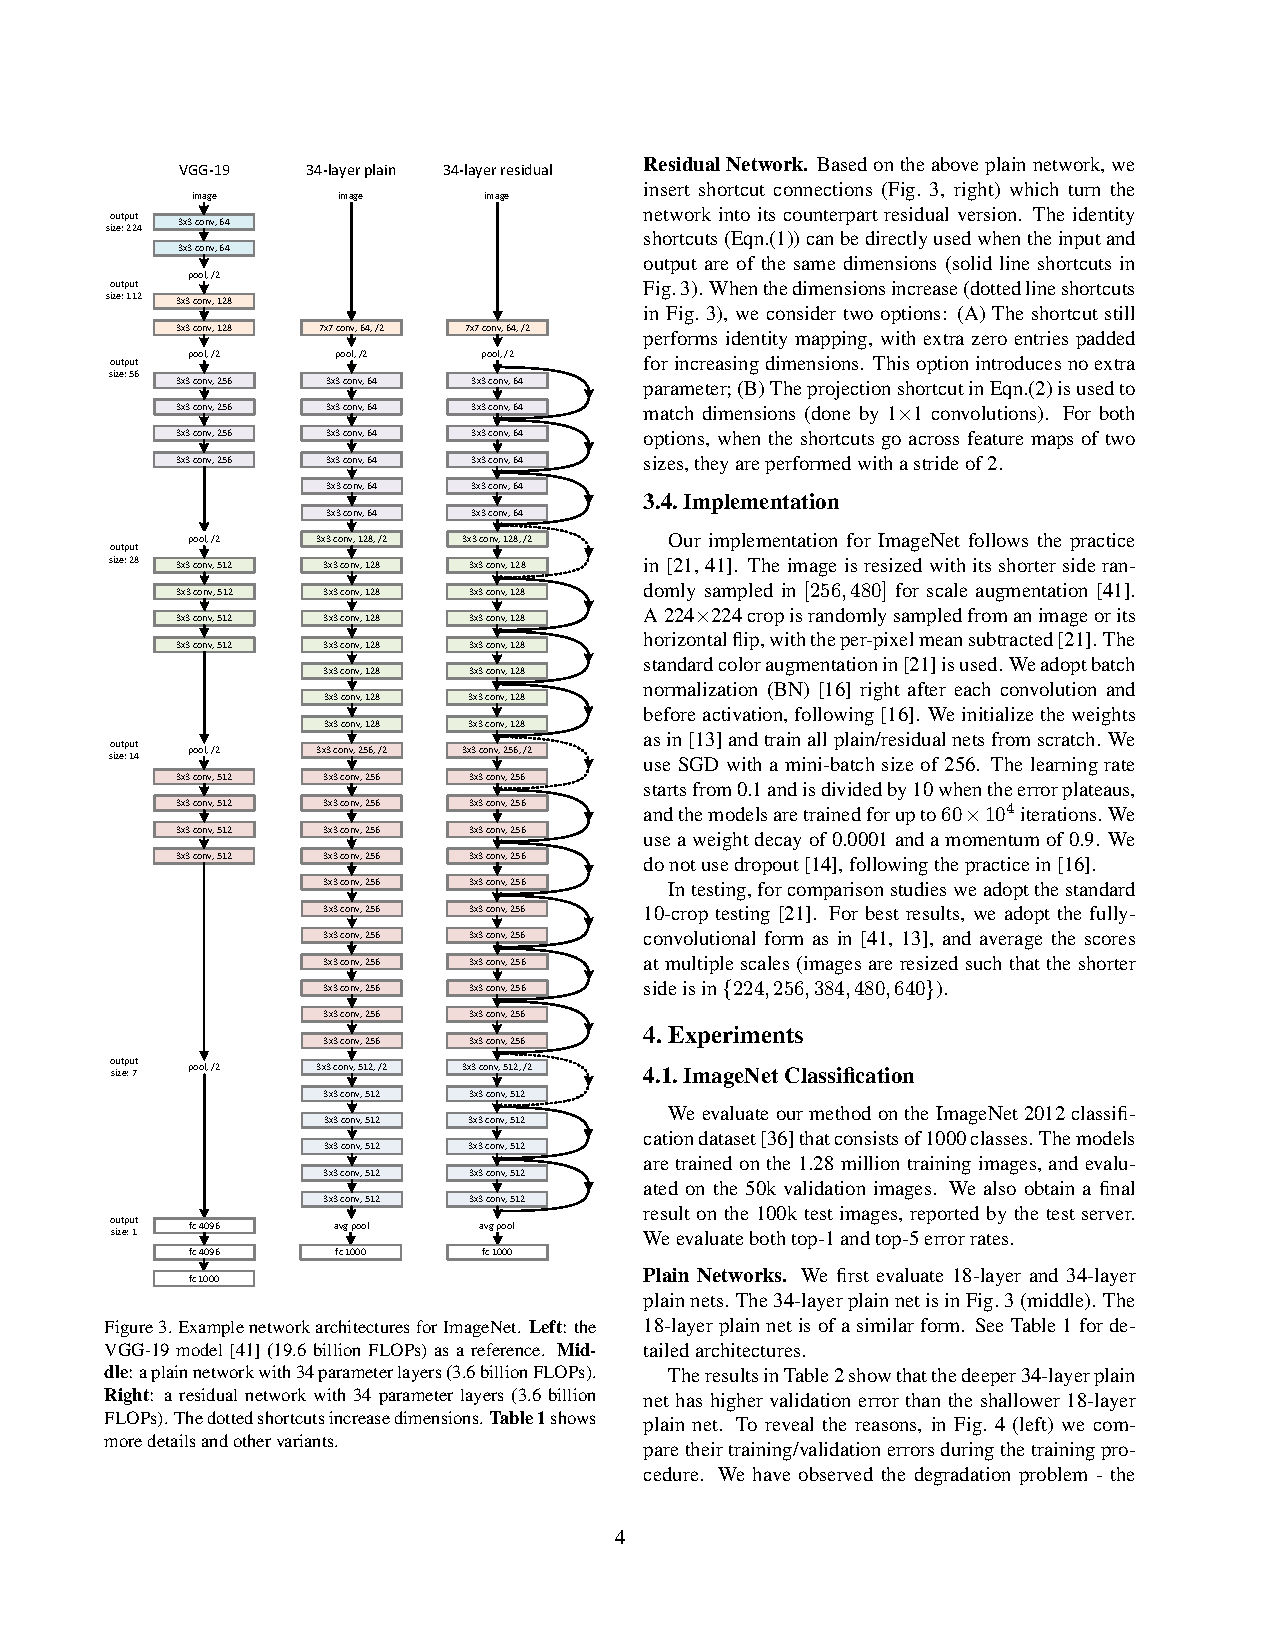
\includegraphics[clip,trim=210 180 320 90,scale=0.35]{excerpts/he_resnet_2015_page_4.pdf}
\\
\acksource{GoogleNet \citep{inception2015}}
&&\acksource{ResNet \citep{he2015resnet}}
\end{tabular}

%--------------------------------------------------

\note[0]{

  Alexnet initiated a trend toward more complex and bigger
  architectures.

  GoogLeNet \citep{inception2015} contains several ``inception''
  modules in a kind of fractal structure.


  Residual networks \citep{he2015resnet} allow very deep networks
  thanks to ``passthrough'' connections which add the input of a layer
  to its output, and facilitate the training.

}

\end{frame}

%%%%%%%%%%%%%%%%%%%%%%%%%%%%%%%%%%%%%%%%%%%%%%%%%%%%%%%%%%%%%%%%%%%%%%

\begin{frame}{}{} %% frame 13 / 53

\makebox[\textwidth][c]{
%% \fbox
{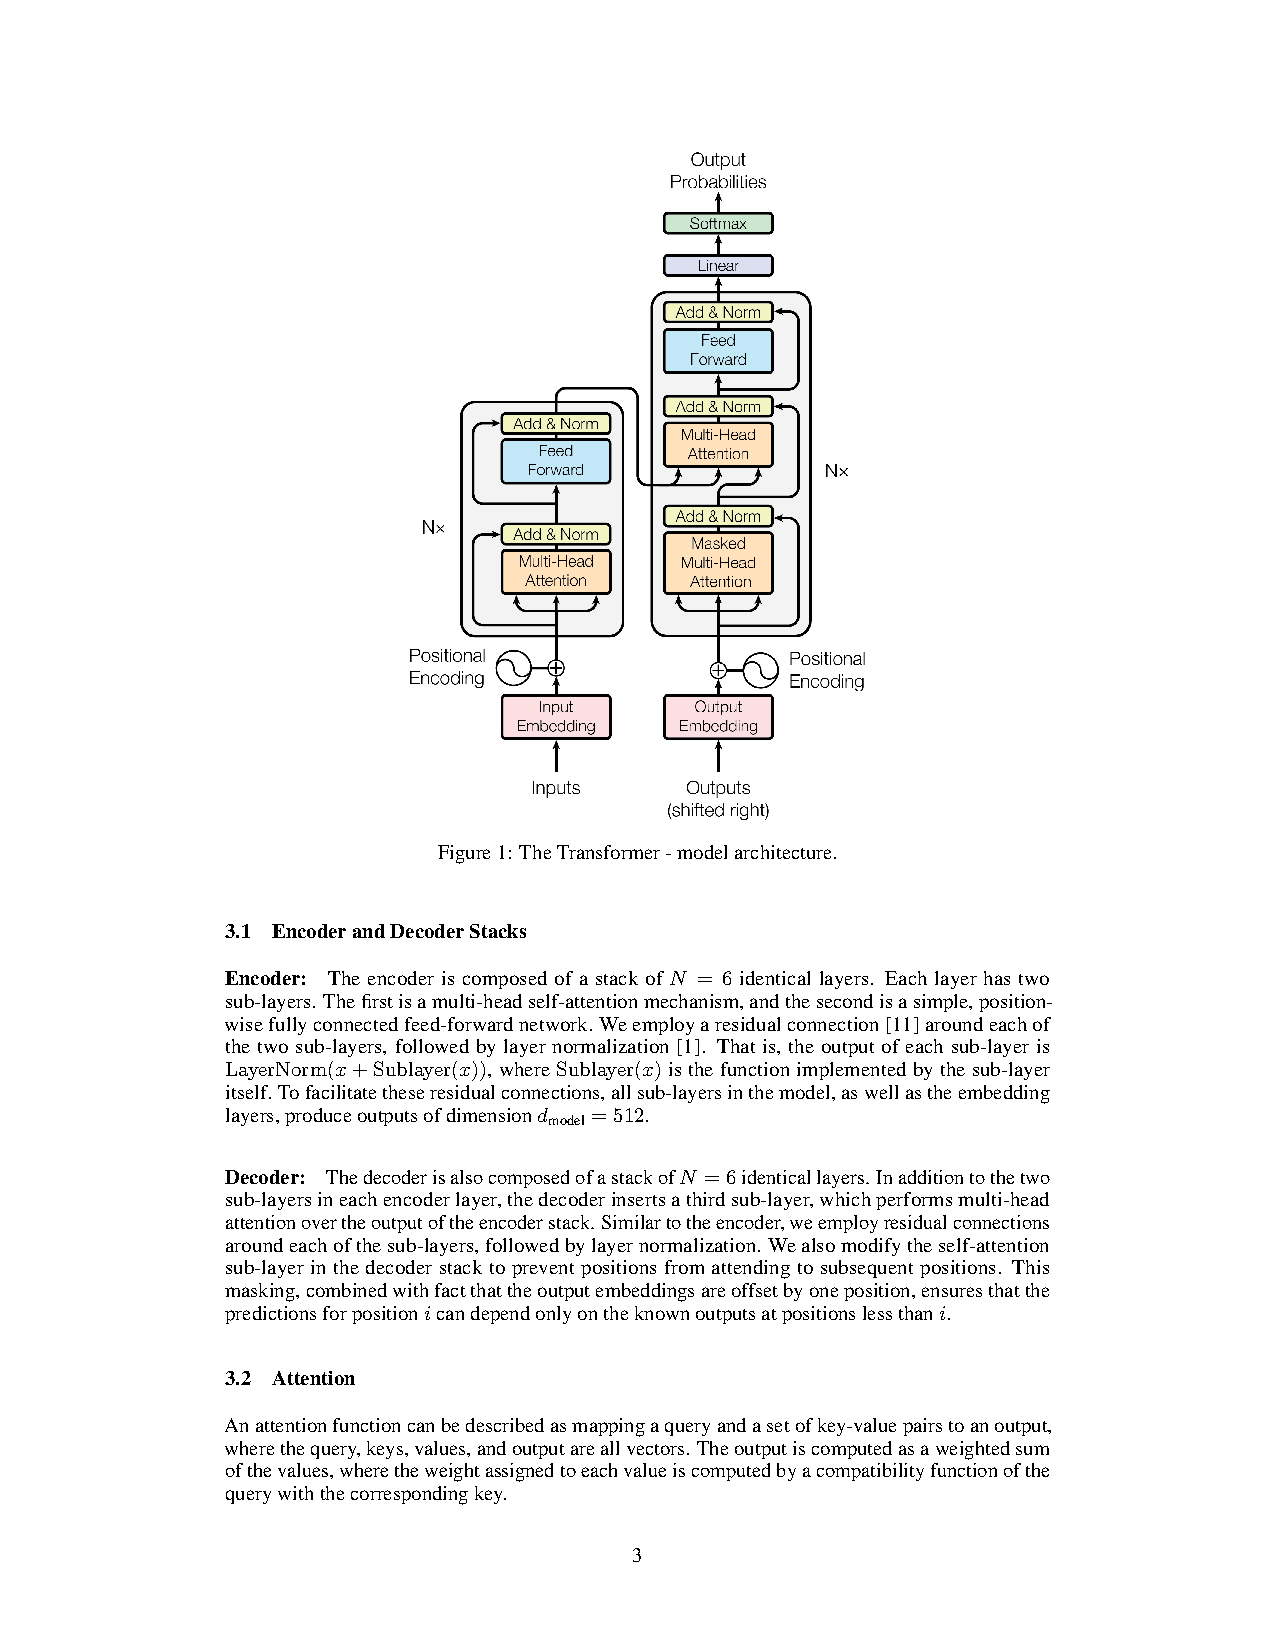
\includegraphics[scale=0.65,trim=190 390 190 70,clip]{excerpts/Vaswani_et_al_2017_3.pdf}}
}

\vspace*{-4ex}

\acksource{\citep{arxiv-1706.03762}}

%--------------------------------------------------

\note[0]{

The Transformers are a class of deep architectures using
attention-based computation, very popular for Natural
Language Processing \citep{arxiv-1706.03762}.

Some of these models for language modeling are of extremely large
size, {e.g.} GPT-3 having 175 billion parameters
\citep{arxiv-2005.14165}.

}

\end{frame}

%%%%%%%%%%%%%%%%%%%%%%%%%%%%%%%%%%%%%%%%%%%%%%%%%%%%%%%%%%%%%%%%%%%%%%

\begin{frame}{}{} %% frame 14 / 53

Deep learning is built on a natural generalization of a neural
network: \textbf{a graph of tensor operators}, taking advantage of
\begin{itemize}
\item the chain rule\index{chain rule} (aka
``back-propagation''\index{back-propagation}),
\item stochastic gradient decent\index{stochastic gradient descent},
\item convolutions,
\item parallel operations on GPUs.\index{GPU}
\end{itemize}

This does not differ much from networks from the 90s.

%--------------------------------------------------

\note[2]{

  As we will see later in the course, an artificial neural network is
  a series of layers of neurons, each neuron connected to several
  neurons in the previous layer and sending activations to neurons
  that follow in the network.

  Deep learning is ``simply'' a natural generalization of artificial
  neural networks by viewing the activities of a group of neurons as a
  multidimensional matrix, called a tensor.

  A ``deep model'' can be formalized as a graph of tensor operators in
  which
  %
  \begin{itemize}
  \item the nodes of the graph are operations,
  \item the results of the operation are propagated along the edges of
    the graph, until it reaches the output node.
  \end{itemize}

  The four main elements of a the deep learning technology are:
  %
  \begin{itemize}

  \item the back-propagation which allows to compute how the quantity
    to optimize will change when changing slightly the model
    parameters. This directly comes from the chain rule from
    differential calculus;

  \item the stochastic gradient descent algorithm, which is a recipe
    to iteratively update the parameters of the network, until it
    fulfills its tasks;

  \item the convolutions, which leverage the fact that the signal is
    structured, and often has some stationarity
    properties. Convolutions allow the processing of large signals
    such as image, videos, or chunks of text. In an image for
    instance, it makes sense to use the same filter detecting an edge
    everywhere;

  \item the parallelization of operations to take advantage of highly
    efficient computing hardware (GPUs/TPUs).

  \end{itemize}

}

\end{frame}

%%%%%%%%%%%%%%%%%%%%%%%%%%%%%%%%%%%%%%%%%%%%%%%%%%%%%%%%%%%%%%%%%%%%%%

\begin{frame}{}{}

This generalization allows to design complex networks of operators
dealing with images, sound, text, sequences, {etc.} and to train them
end-to-end.

%% \includegraphics[width=10cm]{pics/Yeung_et_al_-_End-to-end_Learning_of_Action_Detection_from_Frame_Glimpses_in_Videos_2015_Network-figure.png}

%% \acksource{\citep{arxiv-1511.06984}}

%% \fbox{%
\includegraphics[width=10cm]{pics/Tran_et_al_-_Transform_and_Tell_Entity-Aware_News_Image_Captioning_CVPR_2020_03.png}
%% }

\acksource{\citep{Tran_2020_CVPR}}

%--------------------------------------------------

\note[0]{

  The paradigm of graph of operators allows to design architectures at
  a new level, where submodules themselves perform very complicated
  operations.

  The work of \cite{Tran_2020_CVPR} aims at doing auto captioning from
  images, which is given an input image should produce a piece of text
  describing the content of it. The architecture they devised
  illustrates the modularity of complex deep models, and embeds for
  instance a full ResNet152 as a sub-processing for the image part.

}

\end{frame}

%%%%%%%%%%%%%%%%%%%%%%%%%%%%%%%%%%%%%%%%%%%%%%%%%%%%%%%%%%%%%%%%%%%%%%

%% \begin{frame}{}{} %% frame 18 / 53

%% \vspace*{-0.5cm}

%% %% \fbox{
%% \begin{center}
%% \includegraphics[clip,trim=50 245 320 250,height=7.5cm]{excerpts/he_resnet_2015_page_6.pdf}
%% \end{center}
%% %% }

%% \vspace*{-0.5cm}

%% \acksource{\citep{he2015resnet}}

%% \end{frame}

%% %%%%%%%%%%%%%%%%%%%%%%%%%%%%%%%%%%%%%%%%%%%%%%%%%%%%%%%%%%%%%%%%%%%%%%

%% \begin{frame}{}{} %% frame 24 / 46

%% \begin{center}
%% MS-COCO

%% \includegraphics[height=2.3cm]{pics/mscoco/canvas1_image.jpg}
%% \hspace*{0.1cm}
%% \includegraphics[height=2.3cm]{pics/mscoco/canvas2_image.jpg}
%% \hspace*{0.1cm}
%% \includegraphics[height=2.3cm]{pics/mscoco/canvas5_image.jpg}

%% \includegraphics[height=2.3cm]{pics/mscoco/canvas3_image.jpg}
%% \hspace*{0.1cm}
%% \includegraphics[height=2.3cm]{pics/mscoco/canvas4_image.jpg}
%% \end{center}

%% \end{frame}

%% %%%%%%%%%%%%%%%%%%%%%%%%%%%%%%%%%%%%%%%%%%%%%%%%%%%%%%%%%%%%%%%%%%%%%%

%% \begin{frame}{}{} %% frame 25 / 46

%% \begin{center}
%% MS-COCO

%% \includegraphics[height=2.3cm]{pics/mscoco/canvas1.png}
%% \hspace*{0.1cm}
%% \includegraphics[height=2.3cm]{pics/mscoco/canvas2.png}
%% \hspace*{0.1cm}
%% \includegraphics[height=2.3cm]{pics/mscoco/canvas5.png}

%% \includegraphics[height=2.3cm]{pics/mscoco/canvas3.png}
%% \hspace*{0.1cm}
%% \includegraphics[height=2.3cm]{pics/mscoco/canvas4.png}
%% \end{center}

%% \end{frame}

%%%%%%%%%%%%%%%%%%%%%%%%%%%%%%%%%%%%%%%%%%%%%%%%%%%%%%%%%%%%%%%%%%%%%%

\closingframe

\bibliographyframe

%%%%%%%%%%%%%%%%%%%%%%%%%%%%%%%%%%%%%%%%%%%%%%%%%%%%%%%%%%%%%%%%%%%%%%

\checknbdrafts

\end{document}
